% -*- LaTeX -*-

% PLEASE USE THIS FILE AS A TEMPLATE FOR THE DOCUMENTATION OF YOUR OWN
% FACILITIES: IN PARTICULAR, IT IS IMPORTANT TO NOTE COMMENTS MADE IN
% THE TEXT AND TO FOLLOW THIS ORDERING. THE FORMAT FOLLOWS ONE USED BY
% THE COBE-DMR PROJECT.	
% A.J. Banday, April 1999.

\sloppy

\title{\healpix IDL Facility User Guidelines}
\docid{mollview} \section[mollview]{ }
\label{idl:\thedocid}
\docrv{Version 1.2}
\author{Eric Hivon}
\abstract{This document describes the \healpix facility mollview.}



% q customized for mollview IDL routines
  \newenvironment{qualifiers_mollview}
    {\rule{\hsize}{0.7mm}
     \textsc{\Large{\textbf{QUALIFIERS}}}\hfill\newline%
	\renewcommand{\arraystretch}{1.5}%
	}

% k customized for mollview IDL routines
  \newenvironment{keywords_mollview}
    {\rule{\hsize}{0.7mm}
     \textsc{\Large{\textbf{KEYWORDS}}}\hfill\newline%
	\renewcommand{\arraystretch}{1.5}%
	}

% \usepackage{supertab}

% \newcommand{\layout}{{{p{0.18\hsize} p{0.09\hsize} p{0.70\hsize}}}}
\newcommand{\sizeone}{0.19\hsize}
\newcommand{\sizetwo}{0.08\hsize}
\newcommand{\sizethr}{0.70\hsize}

\begin{facility}
{This IDL facility provides a means to visualise a full sky Mollweide projection of
\healpix and COBE Quad-Cube maps in an IDL environment. 
It also offers the possibility to
generate GIF, JPEG, PDF, PNG and Postscript color-coded images of the projected map. 
The projected (but not color-coded) data can also be output in FITS files and
IDL arrays.}
{src/idl/visu/mollview.pro}
\end{facility}

\newcommand{\mollbacktotop}{\latexhtml{%
%%%%%%\mylink{idl:mollview:TOP}{Back to Format}% for PDF
}{
\mylink{idl:mollview:TOP}{Back to Format}% for HTML
}}
\mytarget{idl:mollview:TOP}%{}


\begin{IDLformat}
{MOLLVIEW, %  File, [Select, ] [/ASINH, CHARSIZE=, COLT=, ... 
%            ... WINDOW=, XPOS=, YPOS= ]
%grep '&' mollview_idl.tex | grep -v hline | grep -v presentation | grep '^{' | awk '{print $1}'
%
\normalsize{
\mylink{idl:mollview:file}{File}, 
[ \mylink{idl:mollview:select}{Select}, ]
[ \mylink{idl:mollview:asinh}{/ASINH}, 
\mylink{idl:mollview:charsize}{CHARSIZE=}, 
\mylink{idl:mollview:charsize}{CHARTHICK=}, 
\mylink{idl:mollview:colt}{COLT=}, 
\mylink{idl:mollview:coord}{COORD=}, 
\mylink{idl:mollview:crop}{/CROP}, 
\mylink{idl:mollview:execute}{EXECUTE=}, 
\mylink{idl:mollview:factor}{FACTOR=}, 
\mylink{idl:mollview:fits}{FITS=}, 
\mylink{idl:mollview:flip}{/FLIP}, 
\mylink{idl:mollview:gal_cut}{GAL\_CUT=}, 
\mylink{idl:mollview:gif}{GIF=}, 
\mylink{idl:mollview:glsize}{GLSIZE=}, 
\mylink{idl:mollview:graticule}{GRATICULE=}, 
\mylink{idl:mollview:half_sky}{/HALF\_SKY}, 
\mylink{idl:mollview:hbound}{HBOUND=}, 
\mylink{idl:mollview:help}{/HELP}, 
\mylink{idl:mollview:hist_equal}{/HIST\_EQUAL}, 
\mylink{idl:mollview:hxsize}{HXSIZE=}, 
\mylink{idl:mollview:iglsize}{IGLSIZE=}, 
\mylink{idl:mollview:igraticule}{IGRATICULE=}, 
\mylink{idl:mollview:log}{/LOG}, 
\mylink{idl:mollview:map_out}{MAP\_OUT=}, 
\mylink{idl:mollview:max}{MAX=}, 
\mylink{idl:mollview:min}{MIN=}, 
\mylink{idl:mollview:nested}{/NESTED}, 
\mylink{idl:mollview:no_dipole}{/NO\_DIPOLE}, 
\mylink{idl:mollview:no_monopole}{/NO\_MONOPOLE}, 
\mylink{idl:mollview:nobar}{/NOBAR}, 
\mylink{idl:mollview:nolabels}{/NOLABELS}, 
\mylink{idl:mollview:noposition}{/NOPOSITION}, 
\mylink{idl:mollview:offset}{OFFSET=}, 
\mylink{idl:mollview:outline}{OUTLINE=}, 
\mylink{idl:mollview:png}{PNG=}, 
\mylink{idl:mollview:polarization}{POLARIZATION=}, 
\mylink{idl:mollview:preview}{/PREVIEW}, 
\mylink{idl:mollview:ps}{PS=}, 
\mylink{idl:mollview:pxsize}{PXSIZE=}, 
\mylink{idl:mollview:pysize}{PYSIZE=}, 
\mylink{idl:mollview:reso_arcmin}{RESO\_ARCMIN=}, 
\mylink{idl:mollview:retain}{RETAIN=}, 
\mylink{idl:mollview:rot}{ROT=}, 
\mylink{idl:mollview:save}{/SAVE}, 
\mylink{idl:mollview:shaded}{/SHADED}, 
\mylink{idl:mollview:silent}{/SILENT}, 
\mylink{idl:mollview:subtitle}{SUBTITLE=}, 
\mylink{idl:mollview:titleplot}{TITLEPLOT=}, 
\mylink{idl:mollview:transparent}{TRANSPARENT=}, 
\mylink{idl:mollview:truecolors}{TRUECOLORS=}, 
\mylink{idl:mollview:units}{UNITS=}, 
\mylink{idl:mollview:window}{WINDOW=}, 
\mylink{idl:mollview:xpos}{XPOS=}, 
\mylink{idl:mollview:ypos}{YPOS=}]
}
}
\end{IDLformat}

% \newcommand{head_column}{{\textbf{name} & \textbf{routine} &
%            \textbf{description}}}

%\vskip 1cm
\mytarget{idl:mollview:routines}%{}
Several visualization routines have a similar interface. Their {\bf qualifiers} and
{\bf keywords} are all listed here, and the routines to which they apply are coded
in the 'routine' column as: \\
A: \htmlref{azeqview}{idl:azeqview},
C: \htmlref{cartview}{idl:cartview},
G: \htmlref{gnomview}{idl:gnomview}, 
M: \htmlref{mollview}{idl:mollview},
O: \htmlref{orthview}{idl:orthview} and all: all of them
%\vskip 2cm 
\vskip 0.4cm

{\bf Qualifiers} should appear in the order indicated. They can take a range of values, and some of them are optional.\\
{\bf Keywords} are optional, and can appear in any order. They take the form {\tt keyword=value} and can be abbreviated to a non ambiguous form
(ie, {\tt factor=10.0} can be replaced by {\tt fac = 10.0}). They generally can take a range of values, but
some of them (noted as {\tt /keyword} below) are boolean switches: they are either present (or set to 1) or absent (or set
to 0).

% \vfill
% \newpage
\begin{qualifiers_mollview}
\begin{tabular}{p{\sizeone} p{\sizetwo} p{\sizethr}}
%% \begin{tabular}{p{0.14\hsize} p{0.08\hsize} p{0.75\hsize}}
\hline  
\textbf{name} & \textbf{routines} & \textbf{\ description} \\ \hline
%                    &   &                            \\ %%% for presentation
File \mytarget{idl:mollview:file}  & \mylink{idl:mollview:routines}{all}   & \parbox[t]{0.95\hsize}{%
		Required\\
                    name of a (possibly gzip compressed) FITS file containing 
               the \healpix\ map in an extension or in the image field, \\
          {\em or}\  \  name of an {\em online} variable (either array or
structure) containing the (RING or \mylink{idl:mollview:polarization}{NESTED} ordered) \healpix\ map (See note below);\\
          if Save is set   :    name of an IDL saveset file containing
               the \healpix\ map stored under the variable  {\tt data} \\
	\nodefault\\
\underline{Note on online data}: in order to preserve the integrity of the input data, 
		the content of the array or structure {\tt File} is replicated
before being possibly altered by the map making process. 
Therefore plotting online data will require more memory than reading the data from disc directly, and is not recommended
		to visualize data sets of size comparable to that of the
computer memory.\\ 
\underline{Note on high resolution cut sky data}: cut sky data (in which less
than 50\% of the sky is observed), can be processed with a minimal memory
foot-print, by not allocating fake full map. In the current release, two
restrictions apply: the input data set must be read from a FITS file in 'cut4'
format, and the \mylink{idl:mollview:polarization}{\tt POLARIZATION} IDL keyword
(described below) must be 0 (default value). See 
\mylink{idl:mollview:example4}{Example \#4} \latexhtml{on page~\pageref{page:example_hires_cutsky}}{below}. \\
\seealso \mylink{idl:mollview:truecolors}{\tt TrueColors}.}\\

Select \mytarget{idl:mollview:select}  & \mylink{idl:mollview:routines}{all}  & \parbox[t]{0.95\hsize}{Optional\\
		  column of the BIN FITS table to be plotted, can be either  \\
                -- a name : value given in TTYPEi of the FITS file \\
                        NOT case sensitive and can be truncated, \\
                        (only letters, digits and underscore are valid) \\
               -- an integer        : number i of the column
                            containing the data, starting with 1 (also valid if
		  \mylink{idl:mollview:file}{{\tt File}} is an online array) \\
                   \default {1 for full sky maps, 'SIGNAL' column for FITS files
		  containing cut sky maps}
               (see the Examples below)}\\

\end{tabular}
\end{qualifiers_mollview}
\vskip 1cm
\mollbacktotop
%======================================================
\newpage
\begin{keywords_mollview}
\begin{tabular}{p{\sizeone} p{\sizetwo} p{\sizethr}}
\hline  
\textbf{name} & \textbf{routines} & \textbf{\ description} \\ \hline
%                    &   &                            \\ %%% for presentation
{ASINH=}\mytarget{idl:mollview:asinh}   & \mylink{idl:mollview:routines}{all}& \parbox[t]{\hsize}{  if set, the
            color table is altered to emulate an non-linear mapping of the input
            data enhancing the low contrast regions. \\
            If {\tt asinh=1} the mapping is $y=\sinh^{-1} (x)$, such that $y \approx x$ when $x\ll 1$ and $y\approx \ln(2x)$ when $x\gg 1$.\\
            If {\tt asinh=2} the mapping is $y=\sinh^{-1} (x/2)/\ln(10)$, such that
$y \approx 0.21 x$ when $x\ll 1$ and $y\approx \log(x)$ when $x\gg 1$. \\
	Here $x$ is the input data, optionally altered by 
	\mylink{idl:mollview:factor}{\tt Factor} and \mylink{idl:mollview:offset}{\tt Offset}. \\
            This option can {\em not} be used in conjonction with
\mylink{idl:mollview:log}{\tt /LOG} nor \mylink{idl:mollview:hist_equal}{\tt /HIST\_EQUAL}.}\\
	

{BAD\_COLOR=}\mytarget{idl:mollview:bad_color}  & \mylink{idl:mollview:routines}{all} & 
\parbox[t]{\hsize}{color given to missing pixels (having
\htmlref{{\tt
!healpix.bad\_value}}{idl:init_healpix} ($=-1.6375\,10^{30}$) 
      or {\tt NaN} value on input).
   The color can be provided as either:\\
    -- a single integer in [0,255], specifying the index to be used in
      the color table chosen via \mylink{idl:mollview:colt}{COLT} (in which the indexes 0, 1 and 2
      are reserved for black, white and grey respectively),\\
    -- a 3 element vector, with each element in [0,255], specifying the
      amount of RED, GREEN and BLUE\\
    -- a 7-character string, starting with '\#', specifying the color in
      HTML Hexadecimal fashion (eg, '\#ff0000' for red).\\
   \default{neutral grey (=2, =[175, 175, 175], ='\#afafaf')}\\
   \seealso \mylink{idl:mollview:bg_color}{BG\_COLOR},
\mylink{idl:mollview:fg_color}{FG\_COLOR}, 
\mylink{idl:mollview:transparent}{TRANSPARENT}} \\
 
{BG\_COLOR=}\mytarget{idl:mollview:bg_color}  & \mylink{idl:mollview:routines}{all}  &  
\parbox[t]{\hsize}{color given to background pixels (outside the sphere).\\
    See \mylink{idl:mollview:bad_color}{BAD\_COLOR} for expected format.\\
    \default{white (=1, =[255, 255, 255], ='\#ffffff')}\\
\seealso \mylink{idl:mollview:fg_color}{FG\_COLOR},
\mylink{idl:mollview:transparent}{TRANSPARENT}}\\

{CHARSIZE=}\mytarget{idl:mollview:charsize}  & \mylink{idl:mollview:routines}{all}  &  
	overall multiplicative factor applied to the size of
        all characters appearing on the plot
        	\default {1.0}; \seealso \mylink{idl:mollview:customize}{CUSTOMIZE} \\ 

{CHARTHICK=}\mytarget{idl:mollview:charthick} & \mylink{idl:mollview:routines}{all}& character thickness (in
\mylink{idl:mollview:titleplot}{TITLEPLOT}, \mylink{idl:mollview:subtitle}{SUBTITLE} and
color bar labeling). Other characters thickness (such as
\mylink{idl:mollview:glsize}{graticule labels}), can be controlled with {\tt !P.CHARTHICK}.
                \default {1} \\

% {COLT=}\mytarget{idl:mollview:colt}  & \mylink{idl:mollview:routines}{all}  & \parbox[t]{\hsize}{ color table number, in [-40,40]. If colt$<0$, the IDL color
%         	table abs(colt) is used, but the scale is
%                reversed (ie a red to blue scale becomes a blue to red
%         	scale). Note: -0.1 can be used as negative 0.\\
%         	\default {33 (Blue-Red)} \\
% \seealso \mylink{idl:mollview:truecolors}{\tt TrueColors}}\\ 

%%%%%%%%%%%%%%%%%
\end{tabular}
\mollbacktotop
%-----------------------------------------------------------
\begin{tabular}{p{\sizeone} p{\sizetwo} p{\sizethr}}
\hline  
\textbf{name} & \textbf{routines} & \textbf{\ description} \\ \hline
%                   &   &                            \\ %%% for presentation
%%%%%%%%%%%%%%%%%

{COLT=}\mytarget{idl:mollview:colt}  & \mylink{idl:mollview:routines}{all}  & \parbox[t]{\hsize}{ color table
index: \\
-- Indexes in [0,40] are reserved for standard IDL color tables, while
  [41,255] are used for user defined color tables read from disc (created and
  written to disc with {\tt MODIFYCT}), if any. \\
-- Indexes 1001 (or {\tt 'planck1'}, case insensitive) and 1002 (or {\tt 'planck2'}) are
reserved for Planck color tables 1 and 2 generated by \htmlref{{\tt
planck\_colors}}{idl:planck_colors}. 
See \mylink{idl:mollview:example6}{Example \#6} \latexhtml{on page~\pageref{page:planck_colors_217}}{below}.\\
-- If the index does not match any existing table, or if it is above 255, 
  the current online table (modifiable with {\tt TVLCT}, {\tt XLOADCT}, {\tt XPALETTE}, ... 
  or eg, J. Davenport's 
\htmladdnormallink%
{{\tt cubehelix.pro}}%
{http://www.astro.washington.edu/users/jrad/cubehelix.pro}
   implementation of D. Green 's
\htmladdnormallink%
{cubehelix color scheme}%
{http://www.mrao.cam.ac.uk/~dag/CUBEHELIX/}%
) is used instead. \\
--If {\tt colt}$<0$, the IDL color table ABS(colt) is used, but the scale is
 reversed (ie a red to blue scale becomes a blue to red scale).
 Note: -0.1 can be used as negative 0.\\
        	\default {33 (Blue-Red)} \\
\seealso \mylink{idl:mollview:truecolors}{\tt TrueColors}}\\ 
%--------


{COORD=}\mytarget{idl:mollview:coord}  & \mylink{idl:mollview:routines}{all}  & \parbox[t]{\hsize}{
		vector with 1 or 2 elements describing the coordinate system of the map;
                either\\
		       -- 'C' or 'Q' : Celestial2000 = eQuatorial, \\
                       -- 'E'        : Ecliptic, \\
                       -- 'G'        : Galactic  \\
               if coord = ['x','y'] the map is rotated from system 'x' to system 'y' \\
               if coord = ['y'] the map is rotated to coordinate system 'y' (with the
               original system assumed to be Galactic unless indicated otherwise in the
                input file) \\
                  \seealso \mylink{idl:mollview:rot}{Rot}}\\


{/CROP}\mytarget{idl:mollview:crop}  & \mylink{idl:mollview:routines}{all}  & \parbox[t]{\hsize}{
		if set, the image produced (in GIF/JPEG/PDF/PNG/PS and on screen) only contains the projected map and
               no title, color bar, ... \\
                \seealso \mylink{idl:mollview:gif}{Gif},
			\mylink{idl:mollview:jpeg}{Jpeg}, 
			\mylink{idl:mollview:pdf}{Pdf},
			\mylink{idl:mollview:png}{Png},
			\mylink{idl:mollview:ps}{Ps}}\\

%%%%%%%%%%%%%%%%%
\end{tabular}
\mollbacktotop
%-----------------------------------------------------------
\begin{tabular}{p{\sizeone} p{\sizetwo} p{\sizethr}}
\hline  
\textbf{name} & \textbf{routines} & \textbf{\ description} \\ \hline
%                   &   &                            \\ %%% for presentation
%%%%%%%%%%%%%%%%%

{CUSTOMIZE=}\mytarget{idl:mollview:customize}  & \mylink{idl:mollview:routines}{all}  & \parbox[t]{\hsize}{User provided structure containing customization parameters of the produced output, whose default values are listed in \mylink{idl:mollview:default_settings}{DEFAULT\_SETTINGS}.
The accepted inputs are \\
{\tt ASPOS.X, ASPOS.Y}: X,Y location of astronomical coordinates label  (which can be removed altogether with \mylink{idl:mollview:noposition}{/NOPOSITION}, only applicable to \htmlref{gnomview}{idl:gnomview}),\\
{\tt CBAR.DX, CBAR.DY}: length and width of color bar (which can be removed with \mylink{idl:mollview:nobar}{/NOBAR}), the bar is centered, at an automatically determined height\\
{\tt CBAR.SPACES}: 3-element vector listing the strings to be inserted between the map minimum value label, the color bar, the map maximum value, and the map units (read from the FITS file or provided by \mylink{idl:mollview:units}{UNITS}) \default{3 single spaces}, \\
{\tt CBAR.TY}: vertical offset of the text (min, max and units labels) with respect to the color bar \default{0};\\
\textbf{Note:} the character size of the text accompanying the color bar is fully determined by the keyword \mylink{idl:mollview:charsize}{Charsize},\\
{\tt CRING.DX, CRING.XLL, CRING.YLL}: radius and X,Y location of lower left corner of the color disc showing the polarization direction when \mylink{idl:mollview:polarization}{POLARIZATION=3}\\
{\tt PDF.DEBUG}: if set to 1, and \mylink{idl:mollview:silent}{SILENT} is not set, then debugging information on the \mylink{idl:mollview:pdf}{PDF} generation will be printed (when applicable), 
and the intermediate Postscript file will be kept\\
{\tt SUBTITLE.X, SUBTITLE.Y, SUBTITLE.CHARSIZE}: control the X,Y location of the plot 
\mylink{idl:mollview:subtitle}{subtitle} 
(X=0 is left justified, X=0.5 is centered and X=1 is right justified), 
and its final character size, which is the product of the number 
{\tt SUBTITLE.CHARSIZE}
with the one provided in the keyword
\mylink{idl:mollview:charsize}{Charsize}\\
{\tt TITLE.X, TITLE.Y, TITLE.CHARSIZE}: same as above, applied to the plot title (\mylink{idl:mollview:titleplot}{titleplot}),\\
{\tt VSCALE.X, VSCALE.Y}: X,Y location of scale calibrating the polarization rods (whose length and spacing in the main plotting area can be tuned with \mylink{idl:mollview:polarization}{POLARIZATION=[3, length, spacing]})\\
See \mylink{idl:mollview:example7}{Example \#7} \latexhtml{on page~\pageref{page:moll_customize}}{below}.
}\\

\hspace{\sizeone}{DEFAULT\-\_SETTINGS=}\mytarget{idl:mollview:default_settings}  & \mylink{idl:mollview:routines}{all}  & \parbox[t]{\hsize}{Structure containing on output the default values (slightly projection dependent) of the plotting parameters that can be customized with 
\mylink{idl:mollview:customize}{CUSTOMIZE}.\\
As shown in \mylink{idl:mollview:example7}{Example \#7} \latexhtml{on page~\pageref{page:moll_customize}}{below}, the returned structure can be inspected with the routine \htmlref{{\tt help\_st}}{idl:help_st}.}\\


%%%%%%%%%%%%%%%%%
\end{tabular}
\mollbacktotop
%-----------------------------------------------------------
\begin{tabular}{p{\sizeone} p{\sizetwo} p{\sizethr}}
\hline  
\textbf{name} & \textbf{routines} & \textbf{\ description} \\ \hline
%                   &   &                            \\ %%% for presentation
%%%%%%%%%%%%%%%%%

{EXECUTE=}\mytarget{idl:mollview:execute}  & \mylink{idl:mollview:routines}{all}  & \parbox[t]{\hsize}{
		character string containing IDL command(s) to be executed in the
plotting window. See 
\mylink{idl:mollview:example3}{Example \#3} \latexhtml{on page~\pageref{page:plot_example_execute}}{below}.}\\
%%\latexhtml{ (on page~\pageref{page:plot_example_execute})}{}}.\\
%%Figure~\ref{fig:plot_example_execute} on page~\pageref{page:plot_example_execute}}\\

{FACTOR=}\mytarget{idl:mollview:factor} & \mylink{idl:mollview:routines}{all}& \parbox[t]{\hsize}{scalar multiplicative factor to be applied to the
	valid data \\
	the data plotted is of the form Factor*(data + Offset) \\
	This does not affect the flagged pixels \\
	Can be used together with ASINH or LOG \\
	When used with TRUECOLORS, FACTOR can be a 3-element vector. \\
        \seealso \mylink{idl:mollview:asinh}{ASINH}, \mylink{idl:mollview:offset}{Offset}, \mylink{idl:mollview:log}{LOG}, \mylink{idl:mollview:truecolors}{Truecolors} \\
	\default {1.0} } \\


{FG\_COLOR=}\mytarget{idl:mollview:fg_color}  & \mylink{idl:mollview:routines}{all}  &  
\parbox[t]{\hsize}{color of title and subtile characters, 
    graticule lines and labels, units, outlines $\ldots$\\
    See \mylink{idl:mollview:bad_color}{BAD\_COLOR} for expected format.\\
    \default{black (=0, =[0, 0, 0], ='\#000000')}\\
   \seealso
\mylink{idl:mollview:bad_color}{BAD\_COLOR},
\mylink{idl:mollview:bg_color}{BG\_COLOR}} \\


{FITS=}\mytarget{idl:mollview:fits} %\hyperdef{cross}{idl:mollview:fits} %
		& \mylink{idl:mollview:routines}{all}& \parbox[t]{\hsize}{
	string containing the name of an output FITS file with
        the projected map in the primary image \\
 	      -- if set to 1            : output the plot in
        plot\_{\em proj}.fits, where {\em proj} is either {\em cartesian, gnomic,
mollweide}, or  {\em orthographic} depending on the projection in use;\\
 	      -- if set to a file name  : output the plot in that file.  \\
 	\default {0: no .FITS done}\\
In the case of Orthographic projection,
\mylink{idl:mollview:half_sky}{HALF\_SKY} must be set.\\
%
Except for the color mapping, all the keywords and options apply to the
projected map, ie: its size is determined by
\mylink{idl:mollview:pxsize}{PXSIZE} (and \mylink{idl:mollview:pysize}{PYSIZE}
when applicable), its angular resolution by \mylink{idl:mollview:reso_arcmin}{RESO\_ARCMIN}
when applicable, its orientation and coordinates by 
\mylink{idl:mollview:rot}{ROT} and 
\mylink{idl:mollview:coord}{COORD} respectively, ... \\
%
	For compatibility with standard FITS viewers (including 
\htmladdnormallink{STIFF}{http://www.astromatic.net/category/softwareposts/stiff})%
, unobserved pixels, and
pixels outside the sphere, take the value {\tt NaN} (ie {\tt !values.f\_nan} in IDL).
The resulting FITS file can be read in IDL with eg. map={\tt readfits}({\em filename}). 
\\
	\seealso \mylink{idl:mollview:map_out}{Map\_out}}\\

{/FLIP}\mytarget{idl:mollview:flip}  & \mylink{idl:mollview:routines}{all}  & if set the longitude increases to the right, whereas by
                default (astronomical convention) it increases towards the left \\
 


{GAL\_CUT=}\mytarget{idl:mollview:gal_cut}  & \mylink{idl:mollview:routines}{---MO}   & (positive float) specifies the symmetric galactic cut in degrees
              outside of which the monopole and/or dipole fitting is done
	\default{0: monopole and dipole fit done on the whole sky}
              (\seealso \mylink{idl:mollview:no_dipole}{No\_dipole}, \mylink{idl:mollview:no_monopole}{No\_monopole}) \\

%%%%%%%%%%%%%%%%%
\end{tabular}
\mollbacktotop
%-----------------------------------------------------------
\begin{tabular}{p{\sizeone} p{\sizetwo} p{\sizethr}}
\hline  
\textbf{name} & \textbf{routines} & \textbf{\ description} \\ \hline
%                   &   &                            \\ %%% for presentation
%%%%%%%%%%%%%%%%%

{GIF=}\mytarget{idl:mollview:gif}  & \mylink{idl:mollview:routines}{all}  & \parbox[t]{\hsize}{
		string containing the name of a .GIF output \\
	      if set to 1            : outputs the plot in 
{\tt plot\_}{\em projection}{\tt .gif}, where {\em projection} is either
{\tt azimequid}, {\tt cartesian}, {\tt gnomic}, {\tt mollweide} 
or {\tt orthographic}, \\
	      if set to a file name  : outputs the plot in that file \\
	Please note that the resulting GIF image might not always look
	      as expected. The reason for this is a problem with
	      'backing store' in the IDL-routine TVRD. Please read the IDL
	      documentation for more information. \\
	\default {no .GIF done} \\              
	\seealso \mylink{idl:mollview:crop}{Crop}, 			
		\mylink{idl:mollview:jpeg}{Jpeg}, 
		\mylink{idl:mollview:pdf}{Pdf}, 
		\mylink{idl:mollview:png}{Png}, 
		\mylink{idl:mollview:preview}{Preview},
		\mylink{idl:mollview:ps}{Ps}
		and \mylink{idl:mollview:retain}{Retain}}\\


{GLSIZE=}\mytarget{idl:mollview:glsize} & \mylink{idl:mollview:routines}{CGMO}& \parbox[t]{\hsize}{
	character size of the graticule labels in units of {\tt Charsize}. \\
        Can be a scalar (which applies to both parallel and meridian labels),
        or a 2 element vector (interpreted as [meridian\_label\_size, parallel\_label\_size])\\
	\default{0: no labeling of graticules}. \\
	\seealso \mylink{idl:mollview:charsize}{Charsize}, \mylink{idl:mollview:graticule}{Graticule},
	\mylink{idl:mollview:iglsize}{Iglsize},
	\mylink{idl:mollview:igraticule}{Igraticule}}\\

{GRATICULE=}\mytarget{idl:mollview:graticule}  & \mylink{idl:mollview:routines}{CGMO}  & \parbox[t]{\hsize}{
	if set, puts a graticule (ie, longitude and latitude grid) 
	in the {\em output} astrophysical coordinates
	with delta\_long = delta\_lat = gdef
         degrees \\
         if set to a scalar $x>$ gmin then delta\_long = delta\_lat = $x$ \\
         if set to [x,y] with $x,y >$ gmin then delta\_long = $x$ and delta\_lat = $y$ \\
          cartview : gdef = 45, gmin =  0 \\
          gnomview : gdef =  5, gmin =  0 \\
          mollview : gdef = 45, gmin = 10 \\
          orthview : gdef = 45, gmin = 10 \\
	Note that the graticule will rotate with the sphere if Rot is set.
	To outline only the equator set graticule=[360,90].
	The automatic labeling of the graticule is controlled by {\tt Glsize}\\
	The graticule line thickness is controlled via !P.THICK.\\
	\default {0 [no graticule]} \\
	\seealso \mylink{idl:mollview:igraticule}{Igraticule}, \mylink{idl:mollview:rot}{Rot}, \mylink{idl:mollview:coord}{Coord}, \mylink{idl:mollview:glsize}{Glsize}
	}\\


{/HALF\_SKY}\mytarget{idl:mollview:half_sky} & \mylink{idl:mollview:routines}{---O} & if set, only shows only one half of the sky 
   (centered on (0,0) or on the location parametrized by \mylink{idl:mollview:rot}{Rot}) instead of the full sky \\
 
%%%%%%%%%%%%%%%%%
\end{tabular}
\mollbacktotop
%-----------------------------------------------------------
\begin{tabular}{p{\sizeone} p{\sizetwo} p{\sizethr}}
\hline  
\textbf{name} & \textbf{routines} & \textbf{\ description} \\ \hline
%                   &   &                            \\ %%% for presentation
%%%%%%%%%%%%%%%%%

{HBOUND=}\mytarget{idl:mollview:hbound} & \mylink{idl:mollview:routines}{all}& scalar or vector of up to 3
elements.
If Hbound[i] is set to a valid $\nside$, the routine will overplot the \healpix\ pixel
boundaries corresponding to that $\nside$
on top of the map. 
The first $\nside$ will be plotted with solid lines, 
the second one (if any) with dashes and
the third one (if any) with dots. Obviously, better results are
obtained for Hbounds elements in growing order.
Since 0-valued boundaries are not plotted, but used for linestyle
assignment, providing Hbound=[0,4] (or [0,0,4]) will
plot $\nside=4$ boundaries with dashes (resp. dots), while Hbound=4 would plot the same
boundaries with solid lines.
\\


{/HELP}\mytarget{idl:mollview:help} & \mylink{idl:mollview:routines}{all}& if set, the routine header is printed (by doc\_library)
      and nothing else is done \\

{/HIST\_EQUAL}\mytarget{idl:mollview:hist_equal}  & \mylink{idl:mollview:routines}{all}  &  \parbox[t]{\hsize}{
		if set,     uses a histogram equalized color mapping
			(useful for non gaussian data field)
		\default {uses linear color mapping and 
                     		puts the level 0 in the middle
                     		of the color scale (ie, green for Blue-Red)
				unless \mylink{idl:mollview:min}{Min} and 
	                               \mylink{idl:mollview:max}{Max} are not symmetric}\\
                     \seealso \mylink{idl:mollview:asinh}{Asinh}, \mylink{idl:mollview:log}{Log}}\\


{HXSIZE=}\mytarget{idl:mollview:hxsize}  & \mylink{idl:mollview:routines}{all}  & \parbox[t]{\hsize}{
		horizontal dimension (in cm) of the \mylink{idl:mollview:ps}{Postscript} printout \\
    		\default {26 cm $\simeq$ 10 in} \\               \seealso \mylink{idl:mollview:pxsize}{Pxsize}}\\

{IGLSIZE=}\mytarget{idl:mollview:iglsize} & \mylink{idl:mollview:routines}{CGMO}& \parbox[t]{\hsize}{
	character size of the input coordinates graticule labels in units of {\tt Charsize}. \\
	Either scalar or 2-element vector (see \mylink{idl:mollview:glsize}{Glsize}).\\
	\default{0: no labeling of graticules}. \\
	\seealso \mylink{idl:mollview:charsize}{Charsize}, \mylink{idl:mollview:igraticule}{Igraticule}
	}\\

{IGRATICULE=}\mytarget{idl:mollview:igraticule}  & \mylink{idl:mollview:routines}{CGMO}  & \parbox[t]{\hsize}{
	if set, puts a graticule (ie, longitude and latitude grid) 
	in the {\em input} astrophysical coordinates.
	See Graticule for conventions and details.
	If both Graticule and Igraticule are set, the latter will
	be represented with dashes.\\
	The automatic labeling of the graticule is controlled by {\tt Iglsize}\\
	\default {0 [no graticule]} \\
	\seealso \mylink{idl:mollview:graticule}{Graticule}, 
\mylink{idl:mollview:rot}{Rot}, \mylink{idl:mollview:coord}{Coord}, 
\mylink{idl:mollview:iglsize}{Iglsize}
	}\\

%%%%%%%%%%%%%%%%%
\end{tabular}
\mollbacktotop
%-----------------------------------------------------------
\begin{tabular}{p{\sizeone} p{\sizetwo} p{\sizethr}}
\hline  
\textbf{name} & \textbf{routines} & \textbf{\ description} \\ \hline
%                   &   &                            \\ %%% for presentation
%%%%%%%%%%%%%%%%%

{JPEG=}\mytarget{idl:mollview:jpeg}  & \mylink{idl:mollview:routines}{all}  & \parbox[t]{\hsize}{
		string containing the name of a {\em lossless} .JPEG output file\\
	      if set to 1            : outputs the plot in 
{\tt plot\_}{\em projection}{\tt .jpeg}, where {\em projection} is either
{\tt azimequid}, {\tt cartesian}, {\tt gnomic}, {\tt mollweide} 
or {\tt orthographic}, \\
	      if set to a file name  : output the plot in that file \\
% 	Please note that the resulting JPEG image might not always look
% 	      as expected. The reason for this is problems with
% 	      'backing store' in the IDL-routine TVRD. Please read the IDL
% 	      documentation for more information. \\
	\default {no .JPEG done} \\              
\seealso 
\mylink{idl:mollview:crop}{Crop}, 
\mylink{idl:mollview:fits}{Fits}, 
\mylink{idl:mollview:gif}{Gif}, 
\mylink{idl:mollview:map_out}{Map\_out}, 
\mylink{idl:mollview:png}{Png}, 
\mylink{idl:mollview:preview}{Preview},
\mylink{idl:mollview:pdf}{Pdf}, 
\mylink{idl:mollview:ps}{Ps}, 
and \mylink{idl:mollview:retain}{Retain}}\\



{LATEX=}\mytarget{idl:mollview:latex}  & \mylink{idl:mollview:routines}{all}  & \parbox[t]{\hsize}{
if set to 1 or 2, enables \LaTeX\ handling of character strings such as 
\mylink{idl:mollview:titleplot}{Titleplot},
\mylink{idl:mollview:subtitle}{Subtitle} and 
\mylink{idl:mollview:units}{Units}\\
        -- if set to 2 {\em with} \mylink{idl:mollview:ps}{PS} or 
          \mylink{idl:mollview:pdf}{PDF} outputs, those strings (and the \mylink{idl:mollview:glsize}{graticule labels}) will be processed 
           by genuine \LaTeX\ and inserted in the final PS or PDF file using {\it psfrag} package
          (requires the ubiquitous \htmladdnormallink{\tt latex}{https://www.ctan.org/starter} and its 
\htmladdnormallink{\it color}{https://www.ctan.org/pkg/color},
\htmladdnormallink{\it geometry}{https://www.ctan.org/pkg/geometry}, 
\htmladdnormallink{\it graphicx}{https://www.ctan.org/pkg/graphicx} and
\htmladdnormallink{\it psfrag}{https://www.ctan.org/pkg/psfrag}
packages as well as \htmladdnormallink{\tt dvips}{https://www.ctan.org/pkg/dvips}).
In this case, the 
\mylink{idl:mollview:pfonts}{Pfonts} settings will be ignored.\\
Note that \htmladdnormallink{\tt cgPStoRASTER}{http://www.idlcoyote.com/programs/cgps2raster.pro},
\htmladdnormallink{ImageMagick {\tt convert}}{http://www.imagemagick.org/script/index.php}
and/or \htmladdnormallink{GraphicsMagick {\tt gm convert}}{http://www.graphicsmagick.org/convert.html}
can be used to turn a PS or PDF file into high resolution GIF, JPEG or PNG file.\\
Beware that the option {\tt latex=2} may not work properly under versions 0.9.5 and older of 
\htmlref{\tt gdl}{install:using_gdl}.\\
        -- if set to 1, with whatever output
(%
\mylink{idl:mollview:gif}{GIF}, 
\mylink{idl:mollview:jpeg}{JPEG},
\mylink{idl:mollview:pdf}{PDF}, 
\mylink{idl:mollview:png}{PNG}, 
\mylink{idl:mollview:ps}{PS}, or X)
LaTeX is partially emulated with \htmladdnormallink{\tt TeXtoIDL}{http://physics.mnstate.edu/craig/textoidl/} routines, which are now shipped with \healpix
          (no extra requirements).	
In this case, \mylink{idl:mollview:pfonts}{Pfonts} settings can be used.\\
	\default{0, no LaTeX handling}	
}\\


{/LOG}\mytarget{idl:mollview:log}  & \mylink{idl:mollview:routines}{all}  & \parbox[t]{\hsize}{
		display the log of map. This is intended for
 	application to positive definite maps only, eg. Galactic foreground
	emission templates; for arbitrary maps, use /ASINH instead.	 \\
	\seealso \mylink{idl:mollview:asinh}{Asinh}, \mylink{idl:mollview:factor}{Factor}, \mylink{idl:mollview:hist_equal}{Hist\_Equal}, \mylink{idl:mollview:offset}{Offset}}\\

{MAP\_OUT=}\mytarget{idl:mollview:map_out} & \mylink{idl:mollview:routines}{all}& \parbox[t]{\hsize}{
	variable that will contain the projected map on output.\\
%
Except for the color mapping, all the keywords and options apply to the
projected map, ie: its size is determined by
\mylink{idl:mollview:pxsize}{PXSIZE} (and \mylink{idl:mollview:pysize}{PYSIZE}
when applicable), its angular resolution by \mylink{idl:mollview:reso_arcmin}{RESO\_ARCMIN}
when applicable, its orientation and coordinates by 
\mylink{idl:mollview:rot}{ROT} and 
\mylink{idl:mollview:coord}{COORD} respectively, ... \\
%
Unobserved pixels, and pixels outside the sphere, take value \htmlref{{\tt
!healpix.bad\_value}}{idl:init_healpix} ($=-1.6375\,10^{30}$).\\
	\seealso \mylink{idl:mollview:fits}{Fits}}\\


%%%%%%%%%%%%%%%%%
\end{tabular}
\mollbacktotop
%-----------------------------------------------------------
\begin{tabular}{p{\sizeone} p{\sizetwo} p{\sizethr}}
\hline  
\textbf{name} & \textbf{routines} & \textbf{\ description} \\ \hline
%                   &   &                            \\ %%% for presentation
%%%%%%%%%%%%%%%%%

{MAX=}\mytarget{idl:mollview:max}  & \mylink{idl:mollview:routines}{all}  & \parbox[t]{\hsize}{
	Set the maximum value for the plotted signal \\ \default{is to use the actual signal
	maximum}.}\\

{MIN=}\mytarget{idl:mollview:min}  & \mylink{idl:mollview:routines}{all}  & \parbox[t]{\hsize}{
	Set the minimum value for the plotted signal \\\default{is to use the actual signal minimum}.}\\	


{/NESTED}\mytarget{idl:mollview:nested}  & \mylink{idl:mollview:routines}{all}  & \parbox[t]{\hsize}{
	specify that the online data is ordered in the nested scheme}\\


{/NO\_DIPOLE}\mytarget{idl:mollview:no_dipole}  & \mylink{idl:mollview:routines}{---MO}   & \parbox[t]{\hsize}{
		if set  (and Gal\_cut is not set) 
                the best fit monopole *and* dipole over all valid pixels are
                removed; \\
                if Gal\_cut is set to $b>0$, the best monopole and dipole fit is performed on all valid
                pixels with $|$galactic latitude$|>b$ (in deg) and is removed from
                all valid pixels \\
	     \default {0 (no monopole or dipole removal)}\\
              can NOT be used together with No\_monopole \\ \seealso {\mylink{idl:mollview:gal_cut}{Gal\_cut}, \mylink{idl:mollview:no_monopole}{No\_monopole}}}\\

{/NO\_MONOPOLE}\mytarget{idl:mollview:no_monopole}  & \mylink{idl:mollview:routines}{---MO}   & \parbox[t]{\hsize}{
		if set (and Gal\_cut is not set) 
                the best fit monopole over all valid pixels is
                removed; \\
                if Gal\_cut is set to $b>0$, the best monopole fit is performed on all valid
                pixels with $|$galactic latitude$|>b$ (in deg) and is removed from
                all valid pixels \\
	     \default {0 (no monopole removal)}\\
              can NOT be used together with No\_dipole \\ \seealso {\mylink{idl:mollview:gal_cut}{Gal\_cut}, \mylink{idl:mollview:no_dipole}{No\_dipole}}}\\


{/NOBAR}\mytarget{idl:mollview:nobar}  & \mylink{idl:mollview:routines}{all}  & if set, the color bar 
(or the color wheel used when \mylink{idl:mollview:polarization}{Polarization}=2) 
is hidden; \seealso \mylink{idl:mollview:customize}{CUSTOMIZE} \\

{/NOLABELS}\mytarget{idl:mollview:nolabels}  & \mylink{idl:mollview:routines}{all}  & if set, color bar labels (min and max) are not present, \default
	{labels are present}; \seealso \mylink{idl:mollview:customize}{CUSTOMIZE}  \\

{/NOPOSITION}\mytarget{idl:mollview:noposition} & \mylink{idl:mollview:routines}{--G--} & if set, the astronomical location of the map
        central point is not indicated; \seealso \mylink{idl:mollview:customize}{CUSTOMIZE}  \\
 


{OFFSET=}\mytarget{idl:mollview:offset} & \mylink{idl:mollview:routines}{all}& \parbox[t]{\hsize}{scalar additive factor to be applied to the valid data \\
	the data plotted is of the form Factor*(data + Offset) \\
	This does not affect the flagged pixels \\
	can be used together with ASINH or LOG \\
	When used with TRUECOLORS, OFFSET can be a 3-element vector. \\
        \seealso \mylink{idl:mollview:asinh}{ASINH}, \mylink{idl:mollview:factor}{Factor}, \mylink{idl:mollview:log}{LOG}, \mylink{idl:mollview:truecolors}{TRUECOLORS} \\
	\default {0.0} } \\
	

%%%%%%%%%%%%%%%%%
\end{tabular}
\mollbacktotop
%-----------------------------------------------------------
\begin{tabular}{p{\sizeone} p{\sizetwo} p{\sizethr}}
\hline  
\textbf{name} & \textbf{routines} & \textbf{\ description} \\ \hline
%                   &   &                            \\ %%% for presentation
%%%%%%%%%%%%%%%%%

{OUTLINE=}\mytarget{idl:mollview:outline} & \mylink{idl:mollview:routines}{CGMO}&  \parbox[t]{\hsize}{
	IDL structure, array of (same size) structures, or structure of (mixed size) structures 
     (see \mylink{idl:mollview:outline:note}{Note below}),  
       containing the description of one (or several) outline(s) to
      be overplotted on the final map.\\
           For each contour or point list, the corresponding (sub)structure should
	contain the following fields:  \\
            -- 'COORD': coordinate system (either 'C'/'Q', 'G' or 'E') of the contour 
           (same meaning as in \mylink{idl:mollview:coord}{Coord})\\
            -- 'RA': RA/longitude coordinates of the contour vertices (array or scalar) \\
            -- 'DEC': Dec/latitude coordinates of the contour vertices (array or
scalar)\\
	and can optionally contain the fields: \\
	    -- 'LINE[STYLE]': (optional, scalar) {\bf +2}: black dashes, {\bf
+1}: black dots, {\bf 0}: black solid (default), {\bf -1}: black dots on white background, {\bf -2}: black dashes on
	white background\\
            -- 'PSY[M]': (optional, scalar) symbol used to represent vertices (same meaning as
	    standard PSYM in IDL. If $9\leq|\mathrm{psym}|\leq 46$, D. Fanning's 
\htmladdnormallink{\tt cgSYMCAT.PRO}{http://www.idlcoyote.com/programs/cgsymcat.pro} symbols 
                     definition will be used; for example, psym=9 is an open circle). If $\leq 0$, the vertices are represented with the chosen symbols, and
                        connected by arcs of geodesics;
                    if $>0$, only the vertices are shown
                    \default {0} \\
            -- 'SYM[SIZE]': (optional, scalar) vertice symbol size (same meaning
as SYMSIZE in IDL), \default {1}\\
	The line and symbol thickness can be controlled (indirectly) via !P.THICK.\\
	Notes: when applicable, the vertices are connected by segments of geodesics. To
	obtain a better looking outline, increase the number of vertices
	provided. The outline does not have to be closed. The procedure will NOT
	attempt to close the outline. See 
\mylink{idl:mollview:example2}{Example \#2} below.
\\{\bf Note:}\mytarget{idl:mollview:outline:note} several outlines 
(let's say {\tt circle} and \mylink{idl:mollview:example2}{{\tt triangle}})
 can be overplotted at once by gathering the respective structures into an array 
({\tt outline=[circle,triangle]}) if they have the same features and in particular the same number of vertices, or in
one meta-structure ({\tt outline=\{s1:circle,s2:triangle\}}) in all cases.\\ \seealso{\mylink{idl:mollview:coord}{Coord}, \mylink{idl:mollview:graticule}{Graticule}}} \\
 

%%%%%%%%%%%%%%%%%
\end{tabular}
\mollbacktotop
%-----------------------------------------------------------
\begin{tabular}{p{\sizeone} p{\sizetwo} p{\sizethr}}
\hline  
\textbf{name} & \textbf{routines} & \textbf{\ description} \\ \hline
%                   &   &                            \\ %%% for presentation
%%%%%%%%%%%%%%%%%

{PDF=}\mytarget{idl:mollview:pdf}  & \mylink{idl:mollview:routines}{all}  &  \parbox[t]{\hsize}{
	      string containing the name of a .PDF output \\
	      if set to 0            : no PDF output \\
	      if set to 1            : outputs the plot in 
{\tt plot\_}{\em projection}{\tt .pdf}, where {\em projection} is either
{\tt azimequid}, {\tt cartesian}, {\tt gnomic}, {\tt mollweide} 
or {\tt orthographic}, \\
	      if set to a file name  : outputs the plot in that file \\
		\default 0 \\
The PDF file is produced from a PostScript file using the script \htmladdnormallink{{\tt epstopdf}}{http://tug.org/epstopdf/} now shipped with \healpixns. Note that {\tt epstopdf} usually requires a fully functional implementation of the fairly widespread {\tt gs}, aka
\htmladdnormallink{{\tt Ghostscript}}{https://en.wikipedia.org/wiki/Ghostscript}, which may however not be available on the computation dedicated nodes of some computer clusters.\\
If the resulting PDF file is not properly rotated (ie landscape orientation instead of portrait), 
and/or has excessive white margins, the scripts
\htmladdnormallink{{\tt pdf90}}{https://linux.die.net/man/1/pdf90}, part of the package 
\htmladdnormallink{{\tt pdfjam}}{http://www2.warwick.ac.uk/fac/sci/statistics/staff/academic-research/firth/software/pdfjam/}, and/or 
\htmladdnormallink{{\tt pdfcrop}}{http://pdfcrop.sourceforge.net}, 
often included in PDFTeX installations, 
can respectively prove very useful.\\
               \seealso 
\mylink{idl:mollview:preview}{Preview}, 
\mylink{idl:mollview:gif}{Gif}, 
\mylink{idl:mollview:jpeg}{Jpeg}, 
\mylink{idl:mollview:png}{Png},
\mylink{idl:mollview:ps}{Ps}}\\


%%%%%%%%%%%%%%%%%
\end{tabular}
\mollbacktotop
%-----------------------------------------------------------
\begin{tabular}{p{\sizeone} p{\sizetwo} p{\sizethr}}
\hline  
\textbf{name} & \textbf{routines} & \textbf{\ description} \\ \hline
%                   &   &                            \\ %%% for presentation
%%%%%%%%%%%%%%%%%

{PFONTS=}\mytarget{idl:mollview:pfonts}  & \mylink{idl:mollview:routines}{all}  &  \parbox[t]{\hsize}{
2-element vector of integers [$p_0$, $p_1$] selecting the default IDL font of character strings such as the
\mylink{idl:mollview:subtitle}{Subtitle},
\mylink{idl:mollview:titleplot}{Titleplot} and
\mylink{idl:mollview:units}{Units}.\\
$p_0$ must be in $\{-1,0,1\}$ and selects the origin of the fonts among
-1: \htmladdnormallink{Hershey Vector}{http://www.exelisvis.com/docs/Using_Hershey_Vector_Fon.html},
0:  \htmladdnormallink{Device Specific}{http://www.exelisvis.com/docs/using_device_fonts.html} and
1:  \htmladdnormallink{True Type}{http://www.exelisvis.com/docs/using_truetype_fonts.html} Fonts.
\\
$p_1$ must be in $\{2,\ldots,20\}$ and selects the starting font of the character strings as described
\htmladdnormallink{here}{http://www.exelisvis.com/docs/Embedded_Formatting_Comm.html}. 
The font can be changed within each string with embedded formatting commands, as discussed on
\htmladdnormallink{\small \tt 
http://www.exelisvis.com/docs/Fonts\_and\_Colors.html}{%
http://www.exelisvis.com/docs/Fonts_and_Colors.html}.\\
\default{[-1,6], corresponding to the Hershey vector font of type 'Complex Roman', and is equivalent to typing
{\tt !p.font=-1} and prepending the
\mylink{idl:mollview:subtitle}{Subtitle},
\mylink{idl:mollview:titleplot}{Titleplot} and
\mylink{idl:mollview:units}{Units} 
strings with {\tt '!6'}}.\\
Note that PFONTS will be ignored if \mylink{idl:mollview:latex}{Latex}=2 {\em and} 
\mylink{idl:mollview:pdf}{PDF} or \mylink{idl:mollview:ps}{PS} are set.
}\\


{PNG=}\mytarget{idl:mollview:png}  & \mylink{idl:mollview:routines}{all}  & \parbox[t]{\hsize}{
		string containing the name of a .PNG output \\
	      if set to 1            : outputs the plot in 
{\tt plot\_}{\em projection}{\tt .png}, where {\em projection} is either
{\tt azimequid}, {\tt cartesian}, {\tt gnomic}, {\tt mollweide} 
or {\tt orthographic}, \\
	      if set to a file name  : outputs the plot in that file \\
	Please note that the resulting PNG image might not always look
	      as expected. The reason for this is problems with
	      'backing store' in the IDL-routine TVRD. Please read the IDL
	      documentation for more information. \\
	\default {no .PNG done} \\              
\seealso 
\mylink{idl:mollview:crop}{Crop}, 
\mylink{idl:mollview:fits}{Fits}, 
\mylink{idl:mollview:gif}{Gif}, 
\mylink{idl:mollview:jpeg}{Jpeg}, 
\mylink{idl:mollview:map_out}{Map\_out}, 
\mylink{idl:mollview:preview}{Preview},
\mylink{idl:mollview:pdf}{Pdf}, 
\mylink{idl:mollview:ps}{Ps}, 
and \mylink{idl:mollview:retain}{Retain}}\\


%%%%%%%%%%%%%%%%%
\end{tabular}
\mollbacktotop
%-----------------------------------------------------------
\begin{tabular}{p{\sizeone} p{\sizetwo} p{\sizethr}}
\hline  
\textbf{name} & \textbf{routines} & \textbf{\ description} \\ \hline
%                   &   &                            \\ %%% for presentation
%%%%%%%%%%%%%%%%%

{POLARIZATION=}\mytarget{idl:mollview:polarization} & \mylink{idl:mollview:routines}{all}& \parbox[t]{\hsize}{
	if set to
	\begin{itemize}
	 \setlength{\itemsep}{0pt}
	 \setlength{\leftmargin}{.1cm}
	 \setlength{\labelwidth}{.1cm}
         \item[0:] no polarization information is plotted;
%
         \item[1:]
             the AMPLITUDE $P = \sqrt{U^2 + Q^2}$ of the polarization is plotted 
	(as long as the input data contains polarization information
             (ie, Stokes parameter $Q$ and $U$ for each pixel));
%
         \item[2:]
             the ANGLE $\phi = \tan^{-1}(U/Q) /2$ of the polarization is plotted \\
             Note: the angles are color coded with a fixed color table (independent of \mylink{idl:mollview:colt}{Colt});
%
         \item[3:]
             --the temperature is color coded (with a color table defined by \mylink{idl:mollview:colt}{Colt}),\\
             --and the polarization is overplotted as headless VECTORS\\
             Polarization can then be a 3-element vector (the first element being 3).
             The second element controls the average length of vectors
             \default{1}, while the third one controls the distance between
             vectors \default{1}. Non-positive values are replaced by 1.
		\seealso \mylink{idl:mollview:customize}{Customize}

	\end{itemize}
	\default{0} \\
	\textbf{Note 1:} The representation of the polarization direction (options 2 and 3 above),
        include the effects of the rotations and/or changes or astronomical coordinates
      (controlled by \mylink{idl:mollview:rot}{ROT} and 
	\mylink{idl:mollview:coord}{COORD} respectively) but do not include the effects
      of the distortions induced by the projection from the sphere to the plan.
      Because the polarization usually has more power at small scales, it must
      generally be represented on maps of small patches of the sky to remain
      legible, in which case the projection-induced distortions are small.\\
	\textbf{Note 2:} when \texttt{polarization=2} or \texttt{polarization=3}, the visualisation routines behavior
     will depend on the value of the \texttt{POLCCONV} FITS keyword
     (see \htmlref{note on POLCCONV}{intro:polcconv} in \linklatexhtml{The \healpix Primer}{intro.pdf}{intro.htm})
	}  \\

%%%%%%%%%%%%%%%%%
\end{tabular}
\mollbacktotop
%-----------------------------------------------------------
\begin{tabular}{p{\sizeone} p{\sizetwo} p{\sizethr}}
\hline  
\textbf{name} & \textbf{routines} & \textbf{\ description} \\ \hline
%                   &   &                            \\ %%% for presentation
%%%%%%%%%%%%%%%%%

{/PREVIEW}\mytarget{idl:mollview:preview}  & \mylink{idl:mollview:routines}{all}  & \parbox[t]{\hsize}{
		if set, the external file generated with \mylink{idl:mollview:gif}{Gif}, 
		\mylink{idl:mollview:jpeg}{Jpeg}, 
		\mylink{idl:mollview:pdf}{Pdf},
		\mylink{idl:mollview:png}{Png},
		or \mylink{idl:mollview:ps}{Ps} will be previewed with the 
		visualisation applications (eg, {\tt gv}, {\tt display} or {\tt open}) 
		chosen during the \htmlref{\healpix IDL/GDL configuration step}{install:idlgdlconfig}}\\

{PS=}\mytarget{idl:mollview:ps}  & \mylink{idl:mollview:routines}{all}  &  \parbox[t]{\hsize}{
	      if set to 0            : no PostScript output \\
	      if set to 1            : outputs the plot 
{\tt plot\_}{\em projection}{\tt .ps}, where {\em projection} is either
{\tt azimequid}, {\tt cartesian}, {\tt gnomic}, {\tt mollweide} 
or {\tt orthographic}, \\
	      if set to a file name  : outputs the plot in that file \\
		\default 0 \\
               \seealso 
\mylink{idl:mollview:preview}{Preview}, 
\mylink{idl:mollview:gif}{Gif}, 
\mylink{idl:mollview:jpeg}{Jpeg}, 
\mylink{idl:mollview:pdf}{Pdf},
\mylink{idl:mollview:png}{Png}}\\


{PXSIZE=}\mytarget{idl:mollview:pxsize}  & \mylink{idl:mollview:routines}{all}  & \parbox[t]{\hsize}{
		set the number of horizontal screen\_pixels or postscript\_color\_dots of the plot
    		(useful for high definition color printer) or elements of the
output map\\
    		\default {800 (Mollview and full sky Orthview), 600 (half sky
		Orthview), 500 (Cartview and Gnomonic)} \\
	\seealso
\mylink{idl:mollview:fits}{FITS}, 
\mylink{idl:mollview:gif}{GIF}, 
\mylink{idl:mollview:jpeg}{JPEG}, 
\mylink{idl:mollview:map_out}{MAP\_OUT}, 
\mylink{idl:mollview:pdf}{PDF},
\mylink{idl:mollview:png}{PNG}, 
\mylink{idl:mollview:ps}{PS}.}\\

{PYSIZE=}\mytarget{idl:mollview:pysize}  & \mylink{idl:mollview:routines}{ACG--}   & \parbox[t]{\hsize}{
		set the number of vertical screen\_pixels or postscript\_color\_dots of the plot \\
    		\default {\mylink{idl:mollview:pxsize}{Pxsize}}.}\\

{RESO\_ARCMIN=}\mytarget{idl:mollview:reso_arcmin} & \mylink{idl:mollview:routines}{ACG--} &  \parbox[t]{\hsize}{
		size of screen\_pixels or postscript\_color\_dots in arcmin \\
        		\default{1.5}\\
	\seealso
\mylink{idl:mollview:fits}{FITS}, 
\mylink{idl:mollview:gif}{GIF}, 
\mylink{idl:mollview:jpeg}{JPEG}, 
\mylink{idl:mollview:map_out}{MAP\_OUT}, 
\mylink{idl:mollview:pdf}{PDF},
\mylink{idl:mollview:png}{PNG}, 
\mylink{idl:mollview:ps}{PS}.}\\

{RETAIN=}\mytarget{idl:mollview:retain} & \mylink{idl:mollview:routines}{all}& \parbox[t]{\hsize}{specifies the type of
backing store to use for direct graphics windows in \{0,1,2\}.
\default{2}. See IDL documentation for details.} \\


{ROT=}\mytarget{idl:mollview:rot}  & \mylink{idl:mollview:routines}{all}& \parbox[t]{\hsize}{
		vector with 1, 2 or 3 elements specifing the rotation angles in DEGREES
               to apply to the map in the 'output' coordinate system (see \mylink{idl:mollview:coord}{Coord})
             = ( lon0, [lat0, rat0])  \\
               lon0 : longitude of the point to be put at the center of the plot
		       the longitude increases Eastward, ie to the left of the plot
 		      \default 0 \\
               lat0 : latitude of the point to be put at the center of the plot
 		      \default 0 \\
               rot0 : anti clockwise rotation to apply to the sky around the
                     center (lon0, lat0) before projecting
                     \default 0 %\\
			%%%\seealso \mylink{idl:mollview:fits}{FITS}%
}\\


%%%%%%%%%%%%%%%%%
\end{tabular}
\mollbacktotop
%-----------------------------------------------------------
\begin{tabular}{p{\sizeone} p{\sizetwo} p{\sizethr}}
\hline  
\textbf{name} & \textbf{routines} & \textbf{\ description} \\ \hline
%                   &   &                            \\ %%% for presentation
%%%%%%%%%%%%%%%%%

{/SAVE}\mytarget{idl:mollview:save}  & \mylink{idl:mollview:routines}{all}  & \parbox[t]{\hsize}{
		if set, assumes that \mylink{idl:mollview:file}{File} is in IDL saveset format, 
    		the variable saved should be DATA} \\
                % can not be used with /ONLINE}\\

{/SHADED}\mytarget{idl:mollview:shaded} & \mylink{idl:mollview:routines}{---O} & \parbox[t]{\hsize}{
		if set, the orthographic sphere is shaded, using a Phong model, to emulate 3D viewing.
              The sphere is illuminated by isotropic ambiant light plus a single light source.
                 Can NOT be used with \mylink{idl:mollview:gif}{GIF}.} \\

{/SILENT}\mytarget{idl:mollview:silent}  & \mylink{idl:mollview:routines}{all}  & \parbox[t]{\hsize}{
		if set, the program runs silently, and extra debugging switches such as 
		\mylink{idl:mollview:customize}{customize=\{pdf:\{debug:1\}\}}
		will be ignored.} \\

{STAGGER=}\mytarget{idl:mollview:stagger}  & \mylink{idl:mollview:routines}{---O}   & \parbox[t]{\hsize}{
Scalar or 2 element vector:\\
            -- if {\tt{stagger[0]}} is in $]0,2]$, 
             three copies of the same sphere centered respectively at {\tt{[-stagger[0], 0, stagger[0]]}}
             (expressed in radius units) along the plot horizontal axis are
             shown in ORTHOGRAPHIC projection\\
             -- if set, {\tt stagger[1]} defines the angle of rotation (in degrees) applied
               to the left and right partial spheres:
             the {\it lhs} sphere is rotated downward by the angle provided,
while the {\it rhs} one
             is rotated upward. Rotations are swapped if \mylink{idl:mollview:flip}{FLIP} is set.\\
Currently {\bf can not} be used with
\mylink{idl:mollview:graticule}{Graticule} nor
\mylink{idl:mollview:igraticule}{igraticule}%
}\\

{SUBTITLE=}\mytarget{idl:mollview:subtitle}  & \mylink{idl:mollview:routines}{all}  & \parbox[t]{\hsize}{
		String containing the subtitle to the plot\\ 
\seealso \mylink{idl:mollview:titleplot}{Titleplot},
\mylink{idl:mollview:latex}{Latex}, \mylink{idl:mollview:customize}{Customize}}\\

{TITLEPLOT=}\mytarget{idl:mollview:titleplot}  & \mylink{idl:mollview:routines}{all}  & \parbox[t]{\hsize}{
		String containing the title of the plot, 
     		if not set the title will be File\\ 
\seealso \mylink{idl:mollview:subtitle}{Subtitle},
\mylink{idl:mollview:latex}{Latex}, \mylink{idl:mollview:customize}{Customize}}\\

{TRANSPARENT=}\mytarget{idl:mollview:transparent}  & \mylink{idl:mollview:routines}{all}  & \parbox[t]{\hsize}{
		If set to 1, the input data pixels with value \htmlref{{\tt
!healpix.bad\_value}}{idl:init_healpix} ($=-1.6375\,10^{30}$) 
will appear totally transparent on the output PNG file (instead of the usual
grey or \mylink{idl:mollview:bad_color}{BAD\_COLOR}).\\ 
If set to 2, the background pixels will be transparent (instead of the usual
white or \mylink{idl:mollview:bg_color}{BG\_COLOR})\\
If set to 3, both the grey and white pixels will look transparent.\\
Active only in conjunction with \mylink{idl:mollview:png}{PNG}}\\

{TRUECOLORS=}\mytarget{idl:mollview:truecolors} & \mylink{idl:mollview:routines}{all}& \parbox[t]{\hsize}{
if the input data is of the form [Npix,3], then the 3 fields
            are respectively understood as {Red, Green, Blue} True-Color
channels, and the \mylink{idl:mollview:colt}{color table} is ignored.\\
-- If set to 1, the mapping field-intensity to color is done for the 3 channels at once. (\seealso \mylink{idl:mollview:factor}{Factor}, \mylink{idl:mollview:offset}{Offset})\\
-- If set to 2, that mapping is done for each channel separately (in that case, \mylink{idl:mollview:min}{MIN}
and \mylink{idl:mollview:max}{MAX} keywords are ignored). 
}\\


%%%%%%%%%%%%%%%%%
\end{tabular}
\mollbacktotop
%-----------------------------------------------------------
\begin{tabular}{p{\sizeone} p{\sizetwo} p{\sizethr}}
\hline  
\textbf{name} & \textbf{routines} & \textbf{\ description} \\ \hline
%                   &   &                            \\ %%% for presentation
%%%%%%%%%%%%%%%%%

{UNITS=}\mytarget{idl:mollview:units}  & \mylink{idl:mollview:routines}{all}  & \parbox[t]{\hsize}{
		String containing the units, to be put on the right
		hand side of the color bar, overrides the value read from the input file,
		if any\\ \seealso \mylink{idl:mollview:nobar}{Nobar}, \mylink{idl:mollview:nolabels}{Nolabels},
\mylink{idl:mollview:latex}{Latex}}\\

{WINDOW=}\mytarget{idl:mollview:window}  & \mylink{idl:mollview:routines}{all}  & \parbox[t]{\hsize}{
                 IDL window index (integer)\\
               -- if WINDOW $< 0$: virtual window: no visible window opened. Can
                 be used with \mylink{idl:mollview:png}{PNG}, \mylink{idl:mollview:jpeg}{JPEG}, 
 or \mylink{idl:mollview:gif}{GIF}, in particular if those files are
larger than the screen. {\bf Note:} The Z buffer will be used instead of the X server,
allowing much faster production of the image over a slow network\\
               -- if WINDOW in $[0,31]$: the specified IDL window with index WINDOW is used
               (or reused). Can be used to have a sequence of images appear
in the same window \\
               -- if WINDOW $> 31$: a free ($=$unused) window with a random index $> 31$ will be
               created and used. \\
	       \default{32, if X server properly set; -1, otherwise}		 
                  }\\

{XPOS=}\mytarget{idl:mollview:xpos}  & \mylink{idl:mollview:routines}{all}  & \parbox[t]{\hsize}{
		The X position on the screen of the lower left corner
	        of the window, in device coordinate}\\

{YPOS=}\mytarget{idl:mollview:ypos}  & \mylink{idl:mollview:routines}{all}  & The Y position on the screen of the lower left corner 
               of the window, in device coordinate

%% %%%%%%%%%%%%%%%%%%%%%%%%%%%%%%%%%%
%% \end{tabular}
%% %--------------------------------------------------------
%% \begin{tabular}{p{\sizeone} p{\sizetwo} p{\sizethr}}
%% \hline  
%% \textbf{name} & \textbf{routines} & \textbf{\ description} \\ \hline



%% \end{tabular}
%% %--------------------------------------------------------
%% \begin{tabular}{p{\sizeone} p{\sizetwo} p{\sizethr}}
%% \hline  
%% \textbf{name} & \textbf{routines} & \textbf{\ description} \\ \hline

\end{tabular}
\mollbacktotop
\end{keywords_mollview}
%***************************************************************

\renewcommand{\projfullname}{{a Mollweide}}
\begin{codedescription}
{
% to be included in codedesciption part of 
% cartview_idl.tex, mollview_idl.tex
% with
%\renewcommand{\projfullname}{a Mollweide}
%\begin{codedescription}
%{
% to be included in codedesciption part of 
% cartview_idl.tex, mollview_idl.tex
% with
%\renewcommand{\projfullname}{a Mollweide}
%\begin{codedescription}
%{
% to be included in codedesciption part of 
% cartview_idl.tex, mollview_idl.tex
% with
%\renewcommand{\projfullname}{a Mollweide}
%\begin{codedescription}
%{\input{mollview_description_idl}}
%\end{codedescription}
{\thedocid{} reads in a \healpix sky map in FITS format and generates
\projfullname \ projection of it, that can be visualized on the screen or
exported in a GIF, JPEG, PNG, PDF or Postscript file. \thedocid{}  allows the selection of
the coordinate system, map size, color table, color bar inclusion,
linear, log, hybrid or histogram equalised color scaling, 
maximum and 
minimum range for the plot, plot-title {\it etc}. It also allows the representation of the
polarization field.}
}
%\end{codedescription}
{\thedocid{} reads in a \healpix sky map in FITS format and generates
\projfullname \ projection of it, that can be visualized on the screen or
exported in a GIF, JPEG, PNG, PDF or Postscript file. \thedocid{}  allows the selection of
the coordinate system, map size, color table, color bar inclusion,
linear, log, hybrid or histogram equalised color scaling, 
maximum and 
minimum range for the plot, plot-title {\it etc}. It also allows the representation of the
polarization field.}
}
%\end{codedescription}
{\thedocid{} reads in a \healpix sky map in FITS format and generates
\projfullname \ projection of it, that can be visualized on the screen or
exported in a GIF, JPEG, PNG, PDF or Postscript file. \thedocid{}  allows the selection of
the coordinate system, map size, color table, color bar inclusion,
linear, log, hybrid or histogram equalised color scaling, 
maximum and 
minimum range for the plot, plot-title {\it etc}. It also allows the representation of the
polarization field.}
}
\end{codedescription}


%
% defines the field 'RELATED' for mollview, gnomview, orthview,
% cartview

\begin{related}
  \begin{sulist}{} %%%% NOTE the ``extra'' brace here %%%%
  \item[idl] version \idlversion or more is necessary to run \thedocid
  \item[ghostview] ghostview or a similar facility is required to view
	  the Postscript image generated by \thedocid.
  \item[xv] xv or a similar facility is required to view the
            GIF/PNG image generated by \thedocid  (a browser can also 
            be used).
  \item[synfast] This \healpix facility will generate the FITS format 
            sky map to be input to \thedocid.
  \item[{\htmlref{cartview}{idl:cartview}}] 
	IDL facility to generate a Cartesian projection of
  	a \healpix map.
  \item[{\htmlref{cartcursor}{idl:cartcursor}}] 
	interactive cursor to be used with cartview
  \item[{\htmlref{gnomview}{idl:gnomview}}] 
	IDL facility to generate a gnomonic projection of
  	a \healpix map.
  \item[{\htmlref{gnomcursor}{idl:gnomcursor}}] 
	interactive cursor to be used with gnomview
  \item[{\htmlref{mollview}{idl:mollview}}] 
	IDL facility to generate a Mollweide projection of
  	a \healpix map.
  \item[{\htmlref{mollcursor}{idl:mollcursor}}] interactive cursor to be used with mollview
  \item[{\htmlref{orthview}{idl:orthview}}] 
	IDL facility to generate an orthographic projection of
  	a \healpix map.
  \item[{\htmlref{orthcursor}{idl:orthcursor}}] 
	interactive cursor to be used with orthview
  \end{sulist}
\end{related}

% defines the field 'RELATED' for mollview, gnomview, orthview,
% cartview

\newpage
\begin{related}
  \begin{sulist}{} %%%% NOTE the ``extra'' brace here %%%%
  \item[idl] version \idlversion or more is necessary to run \thedocid
  \item[gv, ghostview] gv, ghostview or a similar facility is required to view
	  the Postscript or PDF images generated by \thedocid.
  \item[display, xv] display, xv or a similar facility is required to view the
            GIF/JPEG/PNG image generated by \thedocid{} (a browser can also 
            be used).
  \item[\htmlref{synfast}{fac:synfast}, \htmlref{smoothing}{fac:smoothing}] These F90 \healpix facilities will generate the FITS format 
            sky maps to be input to \thedocid.
  \item[\htmlref{isynfast}{idl:isynfast}, \htmlref{ismoothing}{idl:ismoothing}] These IDL routines will generate the FITS format 
            sky maps to be input to \thedocid.
  \item[{\htmlref{cartview} {idl:cartview}}] 
	IDL facility to generate a Cartesian projection of
  	a \healpix map.
  \item[{\htmlref{cartcursor} {idl:cartcursor}}] 
	interactive cursor to be used with cartview
  \item[{\htmlref{gnomview} {idl:gnomview}}] 
	IDL facility to generate a gnomonic projection of
  	a \healpix map.
  \item[{\htmlref{gnomcursor}{idl:gnomcursor}}] 
	interactive cursor to be used with gnomview
  \item[{\htmlref{mollview}{idl:mollview}}] 
	IDL facility to generate a Mollweide projection of
  	a \healpix map.
  \item[{\htmlref{mollcursor}{idl:mollcursor}}] interactive cursor to be used with mollview
  \item[{\htmlref{orthview}{idl:orthview}}] 
	IDL facility to generate an orthographic projection of
  	a \healpix map.
  \item[{\htmlref{orthcursor}{idl:orthcursor}}] 
	interactive cursor to be used with orthview
  \item[{\htmlref{planck\_colors}{idl:planck_colors}}]
        creates color tables used in Planck 2013 publications
  \end{sulist}
\end{related}



%-------------------------------------------
\begin{examples}
{1}
{
\mytarget{idl:mollview:example1}
\begin{tabular}{l} %%%% use this tabular format %%%%
\htmlref{\thedocid}{idl:mollview},  \mylink{idl:mollview:file}{'planck100GHZ-LFI.fits'}, \mylink{idl:mollview:min}{min}=-100, \mylink{idl:mollview:max}{max}=100, \mylink{idl:mollview:graticule}{/graticule}, \$ \\
\hspace{1em}	 \mylink{idl:mollview:titleplot}{title}='Simulated Planck LFI Sky Map at 100GHz'\\
\end{tabular}
}
{\thedocid{} reads in the map 'planck100GHZ-LFI.fits' and generates
an output image in which
the temperature scale has been set to lie between $\pm$ 100 ($\mu$K),
a \mylink{idl:mollview:graticule}{graticule} with a 45 degree step in longitude and latitude is drawn,
and the \mylink{idl:mollview:titleplot}{title} 'Simulated Planck LFI Sky Map at 100GHz' appended to the image.
}
\end{examples}
%-------------------------------------------
\begin{examples}
{2}
{
\mytarget{idl:mollview:example2}
\begin{tabular}{l} %%%% use this tabular format %%%%

map  = findgen(48) \\
triangle= create\_struct('coord','G','ra',[0,80,0],'dec',[40,45,65]) \\
\htmlref{\thedocid}{idl:mollview},\mylink{idl:mollview:file}{map}, \mylink{idl:mollview:graticule}{graticule}=[45,30],\mylink{idl:mollview:rot}{rot}=[10,20,30],\$ \\
\hspace{2em}	  \mylink{idl:mollview:titleplot}{title}='Mollweide projection',\mylink{idl:mollview:subtitle}{subtitle}='mollview', \$ \\
\hspace{2em}          \mylink{idl:mollview:outline}{outline}=triangle \\
\end{tabular}
}
{makes a Mollweide projection of a pixel index map 
(see Figure~\ref{fig:plot_visu}c\latexhtml{ on page~\pageref{page:plot_visu}}{}) after an arbitrary \mylink{idl:mollview:graticule}{rotation}, with a \mylink{idl:mollview:graticule}{graticule} grid
(with a 45$^o$ step in longitude and 30$^o$ in latitude) and an arbitrary
(triangular) \mylink{idl:mollview:outline}{outline}}
\end{examples}
%--------
\begin{figure}[h!]
\latexhtml{%for latex
\centerline{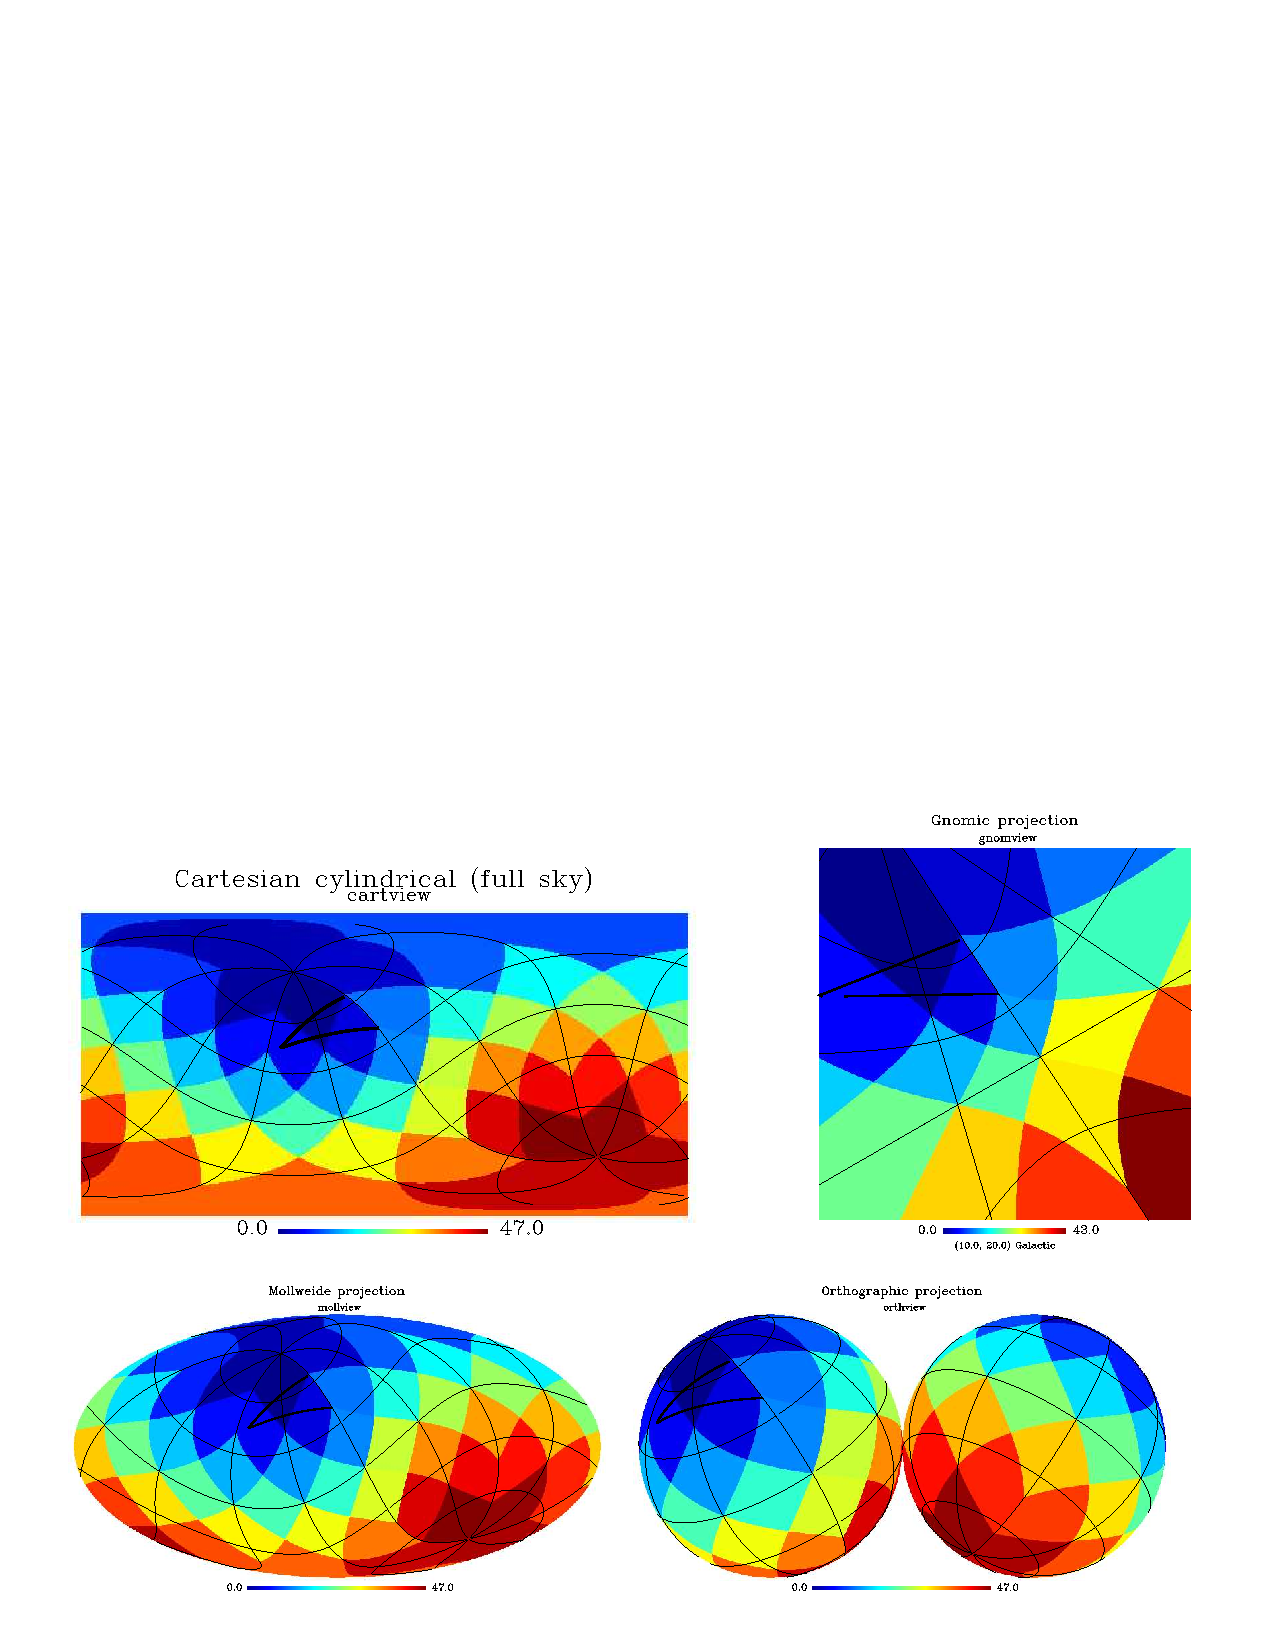
\includegraphics[bb=0pt 0pt 550pt 374pt, width=\textwidth,clip]{fig/merge_visu}}
}{%for html
%\centerline{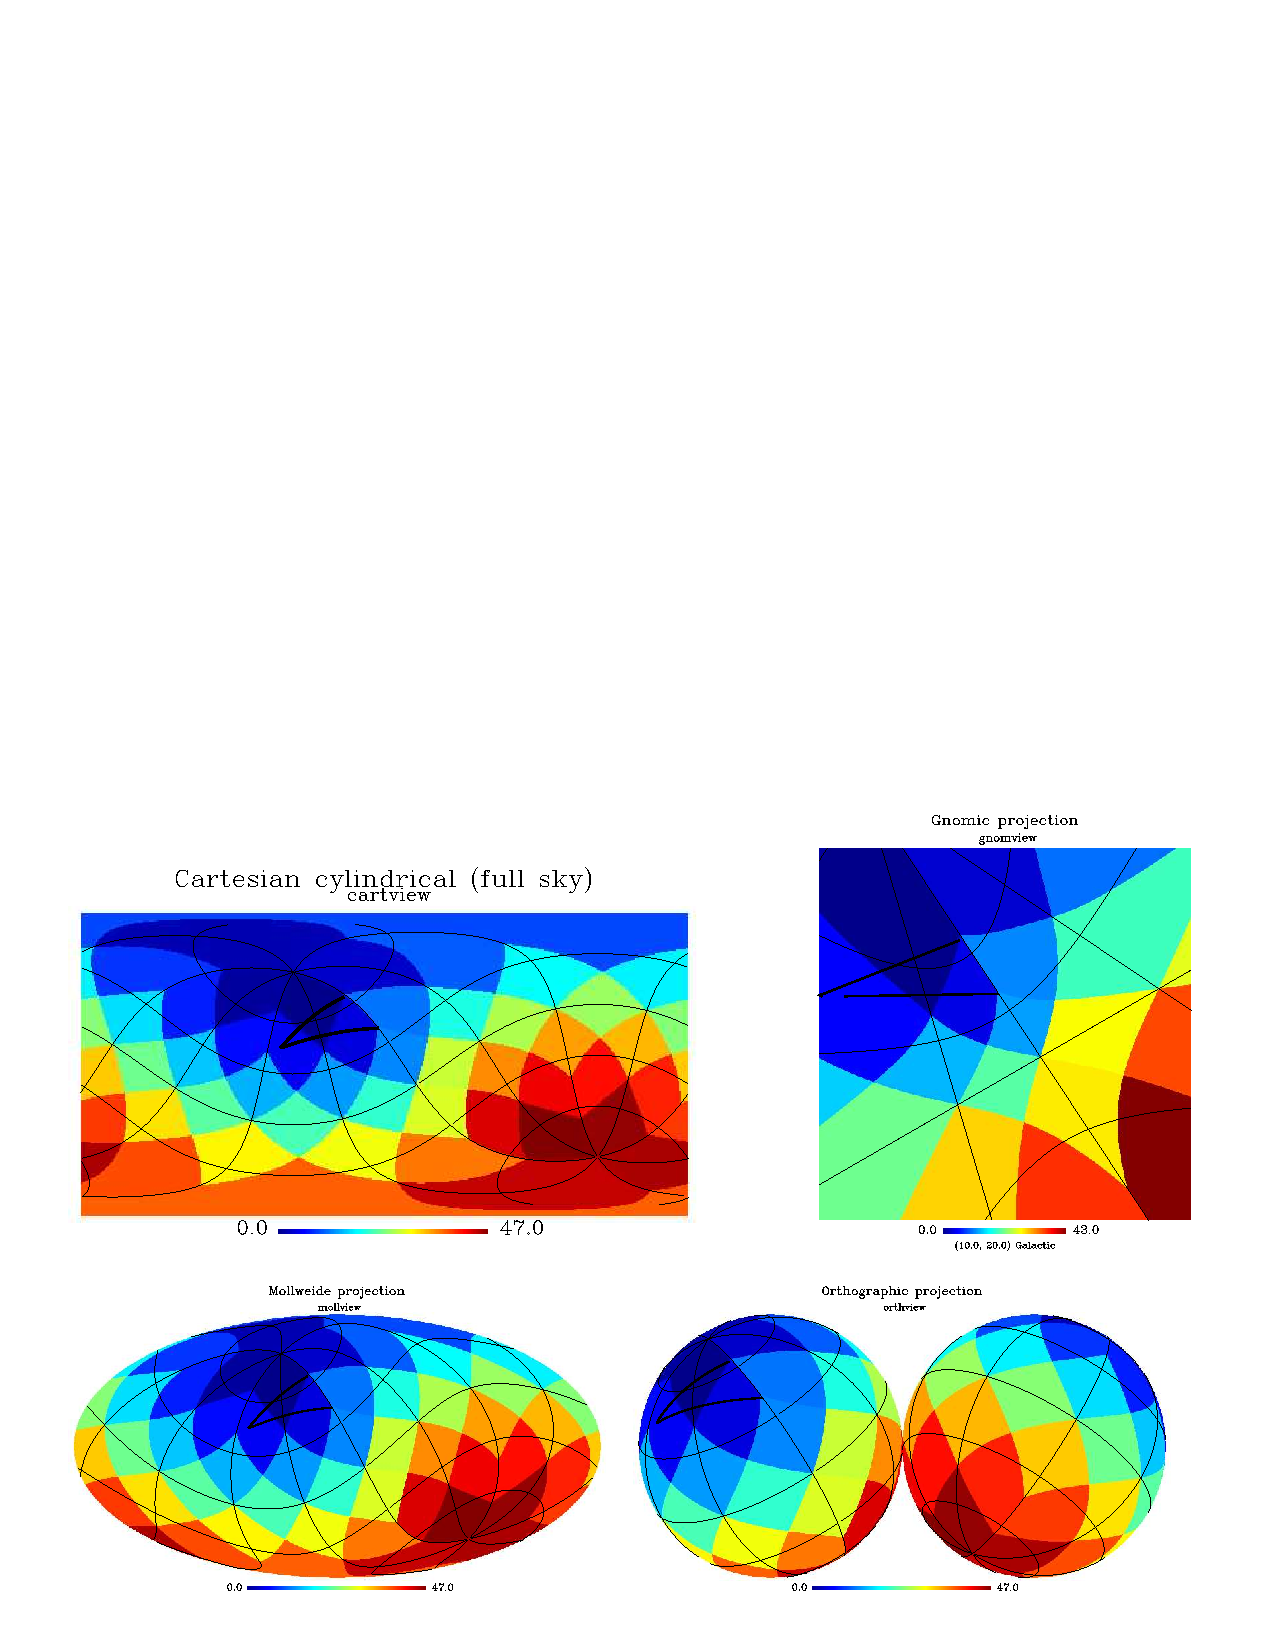
\includegraphics[bb=1pt 1pt 600pt 800pt, width=5in]{fig/merge_visu}\myhtmlimage{}}
%%%\centerline{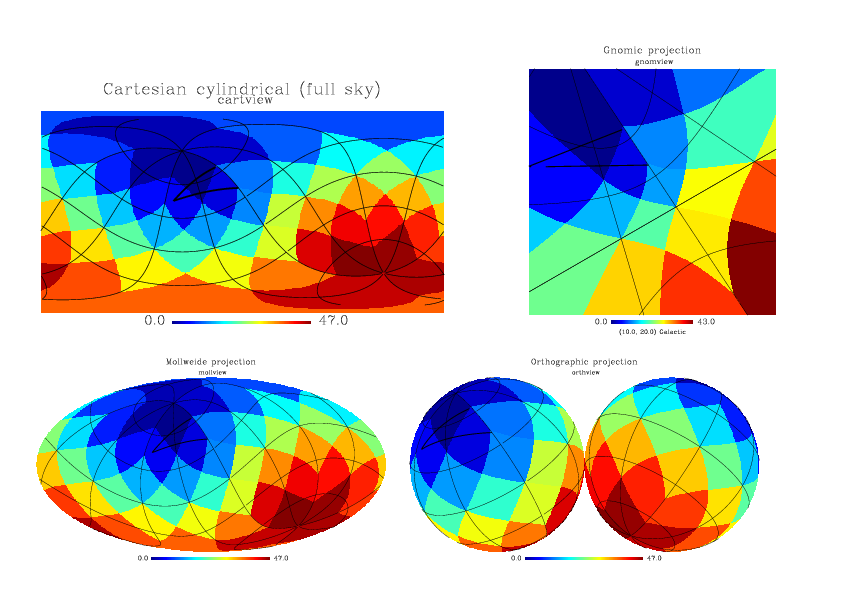
\includegraphics[width=0.5\textwidth]{fig/merge_visu_large}{}}
\centerline{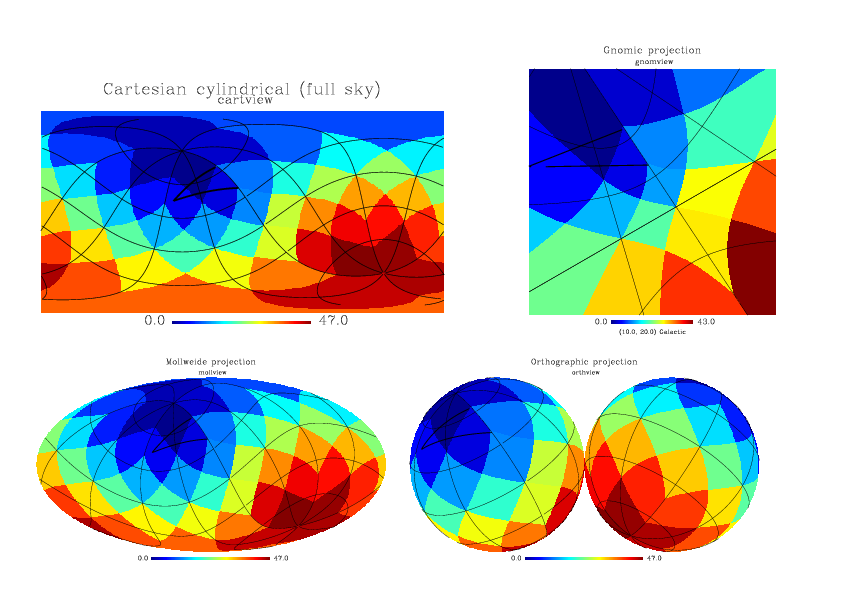
\includegraphics[width=520pt]{fig/merge_visu_large}{}}%rescaled for JPL web site -> ~720
}
\caption{%
\label{page:plot_visu}%
\label{fig:plot_visu}%
Figures produced by \htmlref{cartview}{idl:cartview},
\htmlref{gnomview}{idl:gnomview}, \htmlref{mollview}{idl:mollview} and \htmlref{orthview}{idl:orthview}, see respective
routine documentation for details.}
\end{figure}
%--------

%-------------------------------------------
\begin{examples}
{3}
{
\mytarget{idl:mollview:example3}
\begin{tabular}{l} %%%% use this tabular format %%%%

map  = findgen(48) \\
mycommand = 'x=findgen(64)/10. \& ' + \$ \\
\hspace{2em}	'plot,x,sin(x),pos=[0.8,0.8,0.99,0.99],/noerase \&' +\$ \\
\hspace{2em}	'xyouts,0.5,0.5,''Hello World !'',/normal,charsize=2,align=0.5'  \\
\htmlref{\thedocid}{idl:mollview},map, \mylink{idl:mollview:execute}{execute}=mycommand, \mylink{idl:mollview:png}{png}='plot\_example\_execute.png',\$ \\
\hspace{2em}	\mylink{idl:mollview:preview}{/preview},\mylink{idl:mollview:graticule}{/graticule},\mylink{idl:mollview:glsize}{/glsize} \\
\end{tabular}
}
{produces a PNG file containing a Mollweide projection of a pixel index map
with labeled graticules, a simple sine wave in the
upper right corner, and some greetings, as shown on
Figure~\ref{fig:plot_example_execute}\latexhtml{ on page~\pageref{page:plot_example_execute}}{}%
}
\end{examples}
%-------
\begin{figure}[h!]
\latexhtml{%for latex
\centerline{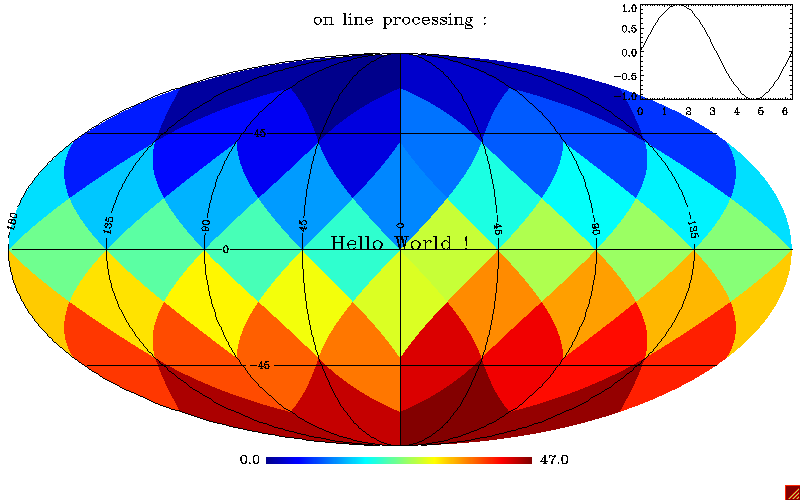
\includegraphics[bb=0pt 20pt 800pt 500pt, width=0.7\textwidth,clip]{fig/plot_example_execute}}
}{%for html
%%%\centerline{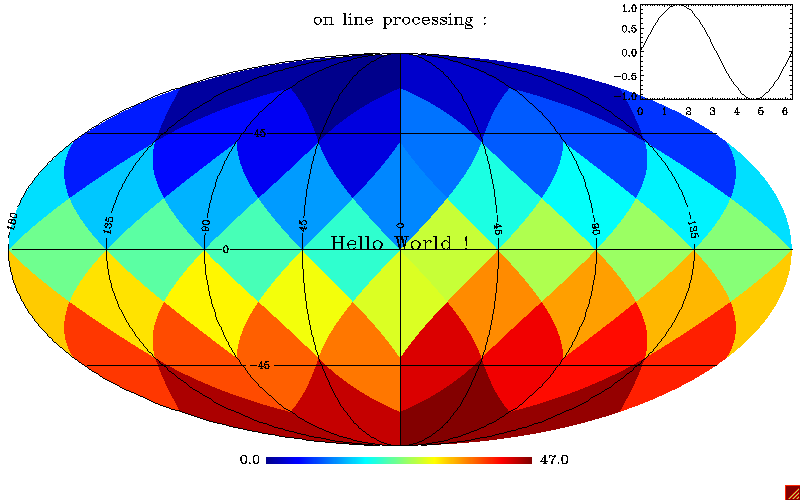
\includegraphics[width=0.5\textwidth]{fig/plot_example_execute}{}}
\centerline{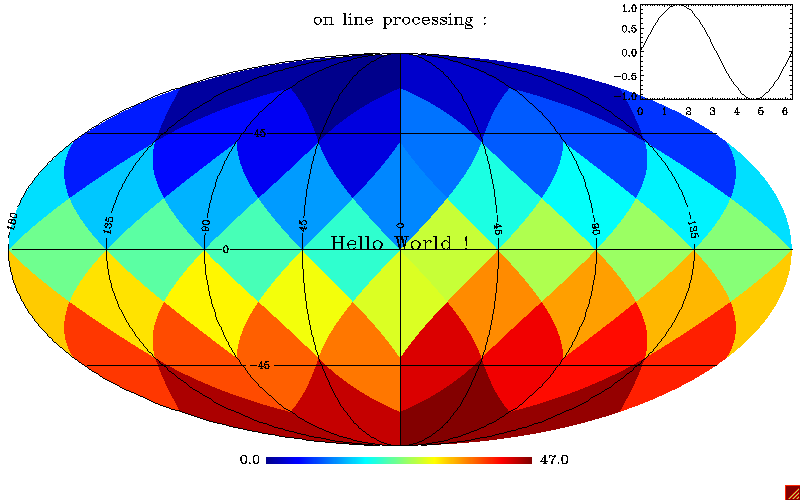
\includegraphics[width=520pt]{fig/plot_example_execute}{}}%rescaled for JPL web site -> ~720
}
\caption{%
\label{page:plot_example_execute}%
\label{fig:plot_example_execute}%
Figure produced by Example \#3 .}
% \mylink{idl:mollview:example3}{Example \#3}.}
\end{figure}
%-------



%-------------------------------------------
\label{page:example_hires_cutsky}
\begin{examples}
{4}
{
\mytarget{idl:mollview:example4}
\begin{tabular}{l} %%%% use this tabular format %%%%

pixel  = l64indgen(400000) \\
signal = pixel * 10.0 \\
file = 'cutsky.fits' \\
\htmlref{write\_fits\_cut4}{idl:write_fits_cut4}, file, pixel+100000, signal, nside=32768, /ring \\
\htmlref{gnomview}{idl:gnomview}, \mylink{idl:mollview:file}{file}, \mylink{idl:mollview:graticule}{rot}=[0,90], \mylink{idl:mollview:graticule}{grat}=30, \mylink{idl:mollview:titleplot}{title}='high res. cut-sky map' \\
\end{tabular}
}
{produces and plots a high resolution map (6.4 arcsec/pixel), in which only a very small subset of
pixels is observed}
\end{examples}
%-------------------------------------------
\begin{examples}
{5}
{
\mytarget{idl:mollview:example5}
\begin{tabular}{l} %%%% use this tabular format %%%%

file = 'wmap\_band\_iqumap\_r9\_5yr\_K\_v3.fits' \\
\htmlref{\thedocid}{idl:mollview}, \mylink{idl:mollview:file}{file}, \mylink{idl:mollview:titleplot}{title}='Linear Color Scale', \mylink{idl:mollview:silent}{/silent} \\
\thedocid, file,\mylink{idl:mollview:asinh}{/asinh},title='Sinh!u-1!n Color Scale' , /silent \\
\thedocid, file,\mylink{idl:mollview:hist_equal}{/hist}, title='Histogram Equalized Color Scale', /silent \\
\thedocid, file,\mylink{idl:mollview:log}{/log},  title='Log Scale', /silent \\
\end{tabular}
}
{produces Mollweide projections of the same map (here the WMAP-5yr K band) with
various color scales: linear, Inverse
Hyperbolic Sine, Histogram Equalized, and Log. See Figure~\ref{fig:merge_wmapKband}%
\latexhtml{ on page~\pageref{page:merge_wmapKband}}{}%
}
\end{examples}
%
\begin{figure}[h!]
\latexhtml{%for latex
%\centerline{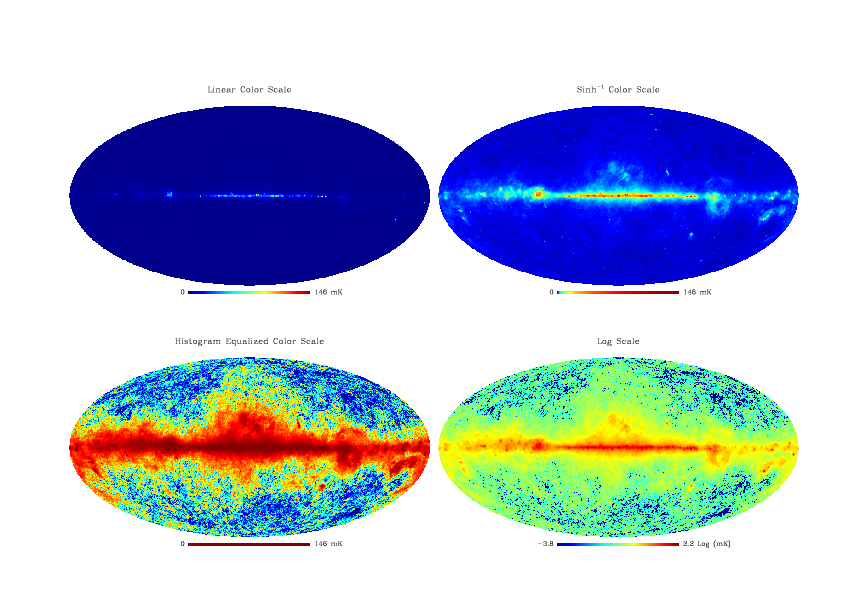
\includegraphics[bb=0pt 0pt 842pt 595pt, width=0.99\textwidth,clip]{fig/merge_wmapKband}}
\centerline{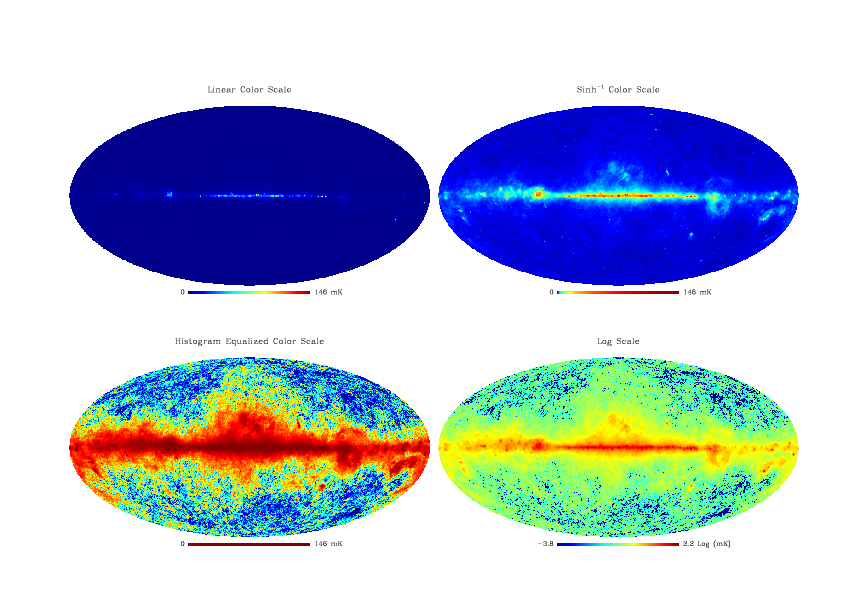
\includegraphics[bb=30pt 40pt 812pt 510pt, width=0.99\textwidth,clip]{fig/merge_wmapKband}}
}{%for html
%%%\centerline{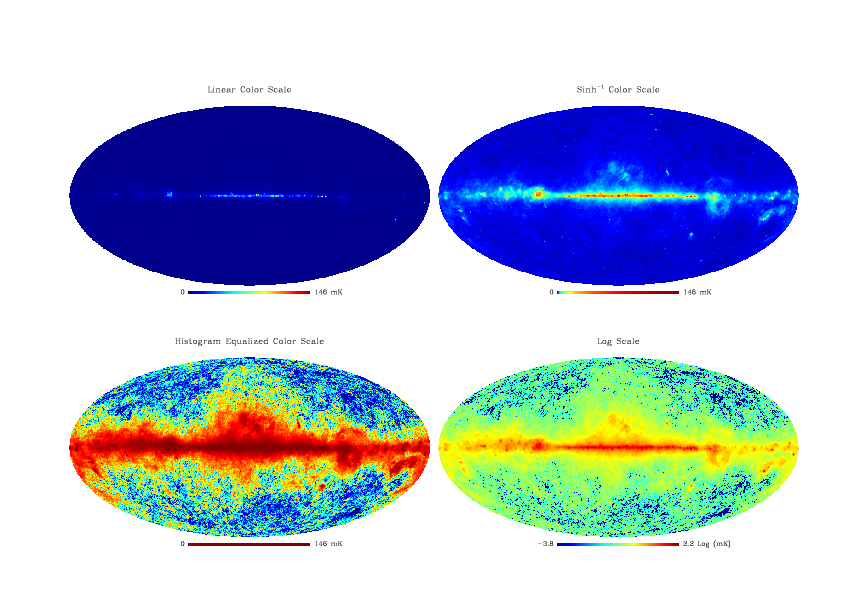
\includegraphics[width=0.5\textwidth]{fig/merge_wmapKband}{}}
\centerline{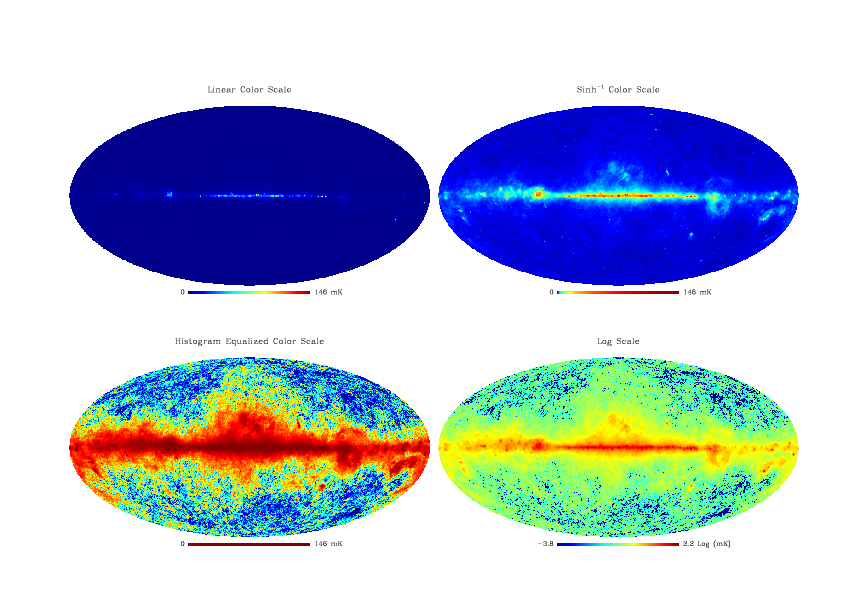
\includegraphics[width=520pt]{fig/merge_wmapKband}{}}%rescaled for JPL web site -> ~720
}
\caption{%
\label{page:merge_wmapKband}%
\label{fig:merge_wmapKband}%
Illustration (generated by 
%\mylink{idl:mollview:example5}{Example~\#5}
Example~\#5)
of the various color scales available.}
\end{figure}

%-------------------------------------------
\newpage
\begin{examples}
{6}
{
\mytarget{idl:mollview:example6}
\begin{tabular}{l} %%%% use this tabular format %%%%
% \thedocid, 2 \\
 \htmlref{mollview}{idl:mollview},
'\htmladdnormallink{HFI\_SkyMap\_217\_2048\_R1.10\_nominal.fits}%
{http://pla.esac.esa.int/pla/aio/planckProducts.html}', \$ \\
\hspace{2em} \mylink{idl:mollview:colt}{colt}='planck2',
\mylink{idl:mollview:asinh}{asinh}=2, 
\mylink{idl:mollview:factor}{factor}=1.e6,
\mylink{idl:mollview:offset}{offset}=-1.33e-4,  \$ \\
\hspace{2em} \mylink{idl:mollview:min}{min}=-1.e3,
\mylink{idl:mollview:max}{max}=1.e7,
\mylink{idl:mollview:titleplot}{title}='Planck @ 217GHz',
\mylink{idl:mollview:charsize}{charsize}=2
\\
\end{tabular}
}
{Illustrates the application of the second color table created by \htmlref{planck\_colors}{idl:planck_colors}  to the
visualization of Planck data at 217GHz 
(see Fig.~\ref{fig:planck_colors_217}\latexhtml{ on page~\pageref{page:planck_colors_217}}{})}
\end{examples}
%
\begin{figure}[h!]
\latexhtml{%for latex
\centerline{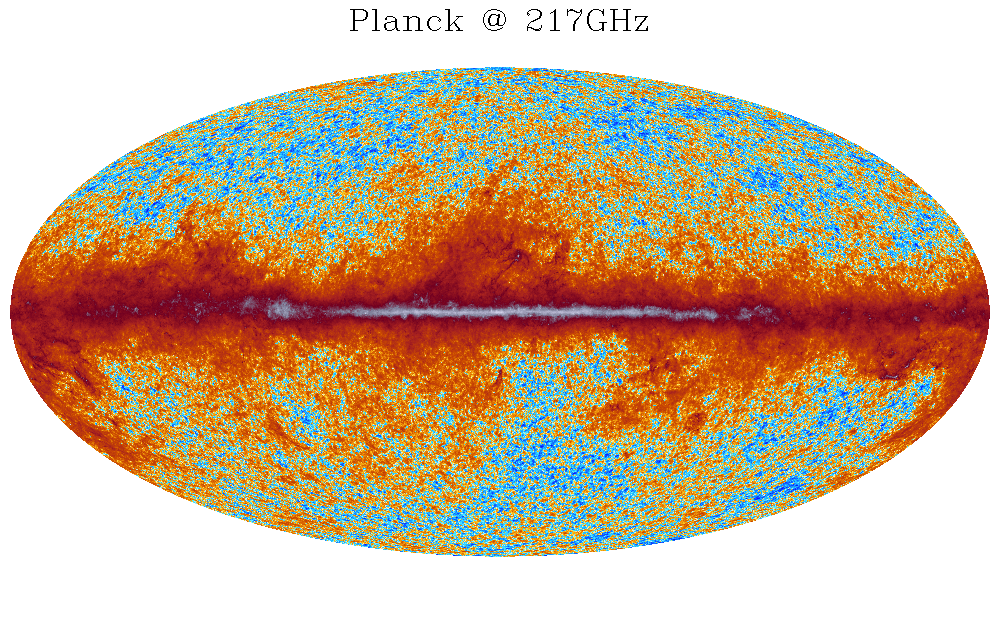
\includegraphics[width=0.99\textwidth]{fig/planck_colors_217}}
}{%for html
\centerline{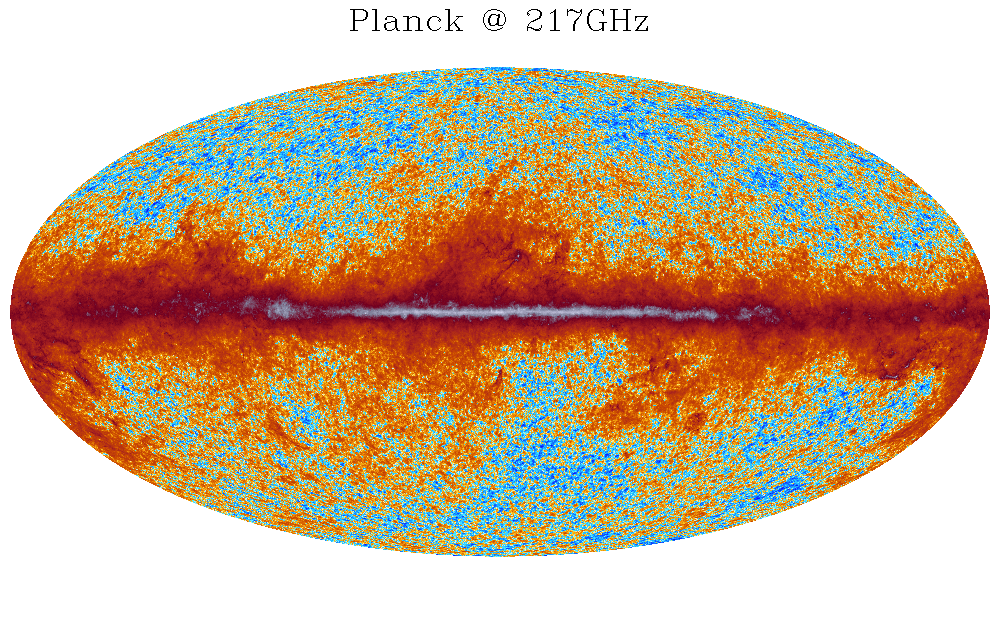
\includegraphics[width=520pt]{fig/planck_colors_217}{}}%rescaled for JPL web site -> ~720
}
\caption{%
\label{page:planck_colors_217}%
\label{fig:planck_colors_217}%
Illustration (generated by 
%\mylink{idl:mollview:example6}{Example~\#6}
Example~\#6) of the application of Planck color table
\#2  to a Planck sky map.}
\end{figure}

%-------------------------------------------
\newpage
\begin{examples}
{7}
{
\mytarget{idl:mollview:example7}
\begin{tabular}{l} %%%% use this tabular format %%%%
 \htmlref{mollview}{idl:mollview}, findgen(12),
 \mylink{idl:mollview:default_settings}{default\_settings=}dsmoll,\$ \\
\hspace{2em} \mylink{idl:mollview:titleplot}{title}=%
'Wider, thicker color bar; left justified title',\$ \\
\hspace{2em}  \mylink{idl:mollview:customize}{customize=}%
\{cbar:\{dx:2/3.,dy:1/32.,ty:0.005\},\$ \\
\hspace{5em}  title:\{x:0,charsize:2\}\} \\
%,png='~/healpix_svn/doc/TeX/fig/moll_customize.png',/preview
 \htmlref{help\_st}{idl:help_st}, dsmoll
\\
\end{tabular}
}
{
\begin{minipage}[t]{\hsize}
will generate a Mollweide projection plot with customized thickness and length of the color bar, 
and location of the title (see Fig.~\ref{fig:moll_customize}\latexhtml{ on page~\pageref{page:moll_customize}}{}). 
The default value (in the Mollweide projection) 
 of the available customization parameters is also listed as \\
{\scriptsize{\texttt{ % put font size before font type to get line spacing right
   ** Structure <4200ac08>, 6 tags, length=120, data length=112, refs=1:\\
\begin{tabular}{lll}
.ASPOS.X                &     FLOAT     &       -1.00000\\
.ASPOS.Y                &     FLOAT     &       -1.00000\\
.CBAR.DX                &     FLOAT     &       0.333333\\
.CBAR.DY                &     FLOAT     &      0.0142857\\
.CBAR.SPACES            &     STRING    &  Array[3]\\
.CBAR.TY                &     FLOAT     &        0.00000\\
.CRING.DX               &     FLOAT     &       0.100000\\
.CRING.XLL              &     FLOAT     &      0.0250000\\
.CRING.YLL              &     FLOAT     &      0.0250000\\
.PDF.DEBUG              &     INT       &      0 \\
.SUBTITLE.X             &     FLOAT     &       0.500000\\
.SUBTITLE.Y             &     FLOAT     &       0.905000\\
.SUBTITLE.CHARSIZE      &     FLOAT     &        1.20000\\
.TITLE.X                &     FLOAT     &       0.500000\\
.TITLE.Y                &     FLOAT     &       0.950000\\
.TITLE.CHARSIZE         &     FLOAT     &        1.60000\\
.VSCALE.X               &     FLOAT     &      0.0500000\\
.VSCALE.Y               &     FLOAT     &      0.0200000
\end{tabular}
}}}
\end{minipage}
}
\end{examples}
%
\begin{figure}[h!]
\latexhtml{%for latex
\centerline{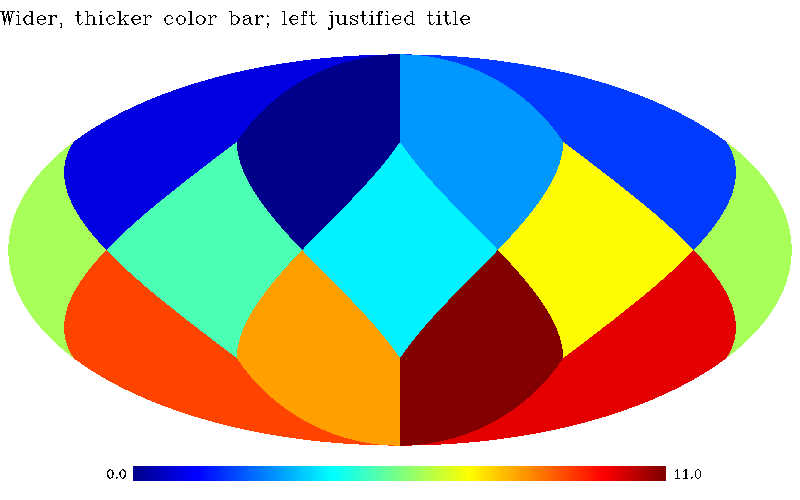
\includegraphics[width=0.49\textwidth]{fig/moll_customize}}
}{%for html
\centerline{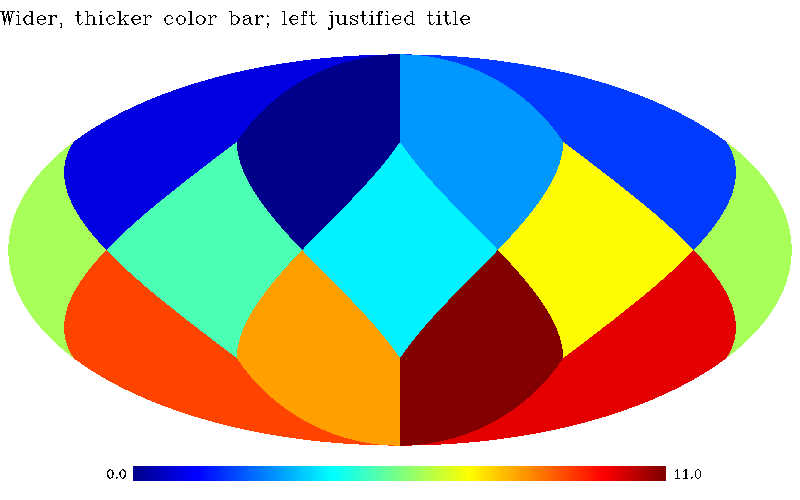
\includegraphics[width=520pt]{fig/moll_customize}{}}
}
\caption{%
\label{page:moll_customize}%
\label{fig:moll_customize}%
Illustration (generated by 
%\mylink{idl:mollview:example7}{Example~\#7}%
Example~\#7
) 
of customization of the title size and location and of the color bar size.}
\end{figure}
%-------------------------------------------

